\documentclass{article}
\usepackage[utf8]{inputenc}
\usepackage[norsk]{babel} 
\usepackage{listings}
\usepackage[sfdefault,light]{roboto}  %font
\usepackage[T1]{fontenc} %font
\usepackage{graphicx} %images
\usepackage[table,xcdraw]{xcolor} %color in tables
\usepackage{array} %tabular: allow multiple lines
\usepackage{longtable} %table that can go over multiple lines
\usepackage{amsfonts} %checkmark
\usepackage{float} %force position
\usepackage{booktabs}
\newcommand{\tabitem}{~~\llap{\textbullet}~~}


\usepackage{geometry} %size of paper
 \geometry{
 a4paper,
 total={170mm,257mm},
 left=25mm,
 right=25mm,
 top=25mm,
 bottom=25mm,
 }

\newcolumntype{L}[1]{>{\raggedright\let\newline\\\arraybackslash}m{#1}} %better looking multirow cells

\usepackage{listings}
\usepackage{color}

\definecolor{dkgreen}{rgb}{0,0.6,0}
\definecolor{gray}{rgb}{0.5,0.5,0.5}
\definecolor{mauve}{rgb}{0.58,0,0.82}

\lstset{frame=tb,
  language=Java,
  aboveskip=3mm,
  belowskip=3mm,
  showstringspaces=false,
  columns=flexible,
  basicstyle={\small\ttfamily},
  numbers=none,
  numberstyle=\tiny\color{gray},
  keywordstyle=\color{blue},
  commentstyle=\color{dkgreen},
  stringstyle=\color{mauve},
  breaklines=true,
  breakatwhitespace=true,
  tabsize=3
}

\begin{document}
\begin{center}
\vspace*{4.5cm}
\Huge{TDT4120}\\[2pc]
\vspace{-1.5cm}
\noindent\rule{11cm}{0.8pt}\\

\Huge{Algoritmer og datastrukturer}\\[1pc]
\vspace{3.5cm}

\Large{2016}\\
%\vspace{1.0cm}
%
\includegraphics[scale=0.6]{images/ntnu.png}
\end{center}

\setlength{\parindent}{3.5em}
%\setlength{\parskip}{1em} % space between index lines
\renewcommand{\baselinestretch}{1.1} % space between lines

\thispagestyle{empty}
\null
\newpage
\setcounter{page}{1}
\pagenumbering{roman}

\tableofcontents
\newpage

\setcounter{page}{1}
\pagenumbering{arabic}

\section{Innleding}
\newenvironment{boxed}
    {\begin{center}
    \begin{tabular}{|p{0.9\textwidth}|}
    \hline\\
    }
    { 
    \\\\\hline
    \end{tabular} 
    \end{center}
    }
\subsection{Hva er algoritmer?}
En algoritme er en hvilket som helst tydelig definert fremgangsmåte for beregninger som kan ta en verdi (eller en mengde verdier) som input og gir en verdi (eller en mengde verdier) som output. Man kan også se på det som et verktøy som skal løse et definert beregningsproblem. Når man definerer problemet, må man beskrive hvilket forhold man ønsker mellom input og output, for eksempel: “Input: Et veikart over en by og to punkter. Output: Den korteste veien (målt i meter) mellom de to punktene.”
\\\\
En algoritme er en veldefinert prosedyre som tar en verdi eller mengde verdier som input og produserer en verdi eller mengde med verdier som output. Dette er en sekvens som transformerer input til output.
At en algoritme er in-place vil si at den opererer på input-dataen uten å måtte lage f.eks. nye arrays for å løse problemet.
\\\\
At en algoritme er stabil vil si at hvis du sorterer en liste med tall, vil alltid tallet i forekomsten som var først i den opprinnelige listen komme først i den sorterte listen.

\subsubsection{Instans}
Hver samling av input-verdier til et problem kalles en instans. For eksempel kan man i en instans av problemet over ha inputverdier som er et veikart over Trondheim, og de to punktene kan være to geografiske punkter som tilsvarer NTNU Gløshaugen og NTNU Dragvoll.

\subsubsection{Problem}
En oppgave generert på generell input. Et problem er en relasjon mellom input og output.

\subsubsection{Probleminstans}
Et problem med et bestemt input. 

\subsubsection{Iterasjon}
En gjennomkjøring av en gjentatt handling.


\newpage
\section{Datastrukturer}

\subsection{Lenkede lister}
En lenket liste er en enkel datastruktur hvor objektene er ordnet lineært. Hvert objekt har helst to peker-variabler; \textit{next} og \textit{prev}. Har den begge disse peker-variablene er det en dobbelt lenket liste. Ved kun en peker (\textit{next}) er det en enkelt-lenket liste. Hvert element peker til det neste i rekkefølgen. Man kan også ha dobbeltlenkede lister, der hver node inneholder en verdi og peker til både forrige og neste node.
\\\\
Vi har forskjellige varianter av lenkede lister, totalt åtte kombinasjoner:
\begin{itemize}
    \item enkle eller doble
    \item sorterte eller usorterte
    \item sirkulære (siste og første element er koblet sammen) eller ikke-sirkulære
\end{itemize}

\begin{lstlisting}
    class Node:
    	def__init__(self):
    		self.value = None
    		self.next = None
    
    n1 = Node()
    n2 = Node()
    n3 = Node()
    n1.value = 1
    n2.value = 2
    n3.value = 3
    n1.next = n2
    n2.next = n3
\end{lstlisting}

\subsubsection{Kjøretider}


\subsection{Abstrakte datastrukturer}
Forkortes ADT.

\subsubsection{Kø}
Kø er en \textbf{FIFO}; first in, first out. En kø implementeres som oftest som et array (gjerne et dynamisk array, likt Java sin ArrayList), men kan også implementeres som en lenket liste. En kø har egenskapene ENQUEUE og DEQUEUE. Det er ingen sniking i en kø, og elementer vil komme ut av køen i samme rekkefølge som de ble lagt inn. Elementer kan legges inn bakerst i køen til enhver tid og man kan når som helst hente ut det første elementet, med mindre køen er tom.

\begin{figure}[H]
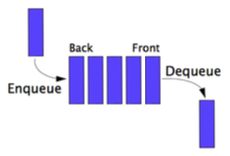
\includegraphics[scale=0.7]{images/ko}
\centering %centering the image
\caption{Queue}
\label{fig:ko}
\end{figure}

\noindent En kø er en abstrakt datastruktur som bevarer de innsatte elementers rekkefølge. Enqueue er innsettingsoperasjonen, som setter inn et element på slutten av køen. Dequeue er uthentingsoperasjonen, den henter ut fra begynnelsen av køen.

\subsection{Stack}
Stack er en \textbf{LIFO}; last in, first out. Det kan sammenlignes med en stabel med tallerkener. Når en tallerken er nyvasket, legges den på toppen. Når du trenger en tar du den øverste i stabelen. Akkurat som at det ikke er lov å snike i en kø, er det ikke lov å stokke om på tallerkenene i en stack. Toppen av stacken er altså det eneste som er tilgjelgelig; du kan når som helst sette inn noe på toppen eller ta ut det øverste elementet (med mindre stacken er tom). En stack implementeres oftest med et array, eller en lenket liste. En stack har egenskapene INSERT, PUSH og POP (DELETE).

\begin{figure}[H]
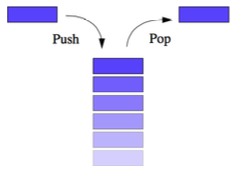
\includegraphics[scale=0.7]{images/stack}
\centering %centering the image
\caption{Stack}
\label{fig:stack}
\end{figure}

\noindent En stakk er en abstrakt datastruktur som, i likhet med en kø, bevarer de innsatte elementers rekkefølge. Siden en stakk er LIFO både legger den til og tar ut fra slutten av strukturen.

\subsection{Heap}
Heaps er den datastrukturen flest har problem med å forstå, samtidig som at det kanskje er den mest nyttige. Styrken til en heap, sammenlignet med en liste, er at den er utrolig rask til å finne det største/minste elementet. Skal man f.eks. be en liste om å finne det minste elementet må man iterere gjennom hele listen, og derfor få en kjøretid på $(n)$. En heap klarer denne oppgaven med kjøretid $O(n log n)$. 
\\\\
En heap er en spesiell tresturktur, som tilfredsstiller heap-egenskapen. Det finnes ingen regler for hvordan søsken er ordnet i heapen. En heap er ofte implementert med et array. Det er viktig å legge merke til at første indeks skal være tom. Det vil si at i et 0-indeksert array vil plass 0 være tom, mens første node står på indeks 1.

\begin{table}[H]
    %\caption{}
    \label{tab:datastrukturer}
    \centering
    \begin{tabular}{|L{15em} | L{15em}|}
        \hline
        \rowcolor[HTML]{303F9F}
        \textbf{\textcolor{white}{Operasjon}} & \textbf{\textcolor{white}{ Tidskompleksitet}}\\
        \rowcolor[HTML]{E6E6E6}
        Finn min/max & $\theta(1)$\\
        Slett min/max & $\theta(log n)$\\
        \rowcolor[HTML]{E6E6E6}
        Sett inn & $\theta(log n)$\\
        Omstrukturere heap & $\theta(log n)$\\
         \rowcolor[HTML]{E6E6E6}
        Merge & $\theta(n)$\\
         \hline
    \end{tabular}
\end{table}

\noindent Måten en heap fungerer på er nesten litt ”magisk”. Ved å alltid la hver node i et binærtre ha en egenskap, så får man automagisk en heap. Denne egenskapen er: elementene som er direkte under noden har lavere verdi enn noden.

\begin{table}[H]
    %\caption{}
    \label{tab:heap}
    \centering
    \begin{tabular}{|L{10em} | L{10em}| L{10em}|L{10em}|}
        \hline
        \rowcolor[HTML]{303F9F}
        \textbf{\textcolor{white}{}} & \textbf{\textcolor{white}{Lenket liste}} & \textbf{\textcolor{white}{Array}} & \textbf{\textcolor{white}{Dynamisk array}}\\
        \rowcolor[HTML]{E6E6E6}
        Indeksering & $\theta(n)$ & $\theta(1)$ & $\theta(1)$\\
        Ins/del front & $\theta(1)$ & - & $\theta(n)$\\
        \rowcolor[HTML]{E6E6E6}
        Ins/del bakerst & $\theta(n)$ & - & $\theta(1)$\\
        Ins/del midten & $Søk + \theta(1)$ & - & $\theta(n)$\\
         \rowcolor[HTML]{E6E6E6}
        Unrukt plass & $\theta(n)$ & 0 & $\theta(n)$\\
         \hline
    \end{tabular}
\end{table}

\noindent I en heap må hele treet være fullstendig fylt ut, bortsett fra muligens det laveste nivået, som fylles ut fra venstre.
\begin{itemize}
    \item Rotnode: $i = 1$
    \item Foreldrenode(i): $i/2$
    \item Høyre-barn: $(2i + 1)$
    \item Venstre-barn: $(2i)$
\end{itemize}

\subsubsection{Max-heap}
For hver node $i$, bortsett fra rot-noden, må verdien til barnenodene være mindre eller lik foreldrenoden. $A[PARENT(i)]\geq A[i]$

\subsubsection{Min-heap}
For hver node $i$, bortsett fra rot-noden, må verdien til barnenodene være større eller lik foreldrenoden. $A[PARENT(i)]\leq A[i]$




\newpage
\section{Kjøretidsberegning}
\subsection{Om kjøretider}
For å vite hvor effektiv en algoritme er, ønsker man å vite hvor kjapp den er i forhold til hvor mye informasjon man sender inn. Noen ganger vil en dobling av antall inn-verdier bare øke kjøretiden med en konstant tid, andre ganger vil den doble kjøretiden, og ofte vil den øke med veldig mye.
\\\\
Kjøretider skal alltid oppgis med \textbf{asymptotisk notasjon}. Det vil si at man finner (teoretisk) matematisk funksjon for kjøretiden med antall inn-verdier som parameter. Deretter ser man på det leddet som dominerer mest i uttrykket når inn-verdiene blir store nok, og bruker dette (uten noe konstantledd) som et mål på hvor rask algoritmen er. Målet er at det ikke skal vokse særlig raskt.

\begin{boxed}
Anta at du har mange forskjellige tall, og du skal finne det største taller. Du sjekker da det første tallet, og setter denne som en midlertidig mulighet for at det er det største tallet. Deretter går du gjennom resten av tallene og sammenligner hver og en av dem med det tallet du antar er det største. Hvis du plukker opp et større tall enn du har fra før, setter du det nye til å være en mulighet for å være det største. Når du har gått gjennom alle tallene, vil det tallet du satte av som en mulig kandidat sist være det største tallet. Slik må det være, fordi da du plukket opp det største tallet satte du dette som en mulig kandidat og ingen andre tall var større. Dette gjelder selvsagt også om flere tall er like i verdi. Så lenge du ikke kunne ane hvor i bunken det største er da du begynte, vet du at du er nødt til å gå gjennom alle tallene en gang.
\newline \newline
På en andre siden trenger du ikke gå gjennom tallene flere ganger heller, for ved å bruke algoritmen beskrevet ovenfor, vet du at svaret er korrekt etter nøyaktig en gjennomgang (så lenge du ikke gjør noen feil underveis, vel og merke!). Hvis mengden med tall dobles og du antar at du alltid vil bruke like lang tid på hver sammenligning uansett hvor mange tall du har, vil arbeidstiden også dobles. Det kan f.eks. se slik ut:
\newline \newline
Du har tallene 2 3 1 7 5
\newline \newline
1. steg: Du sjekker tallet 2; 2 er nå kandidat til å være det største tallet.\\
2. steg: Du sjekker tallet 3; 3 er nå kandidat til å være det største tallet.\\
3. steg: Du sjekker tallet 1; 3 er fortsatt størst.\\
4. steg: Du sjekker tallet 7; 7 er nå kandidat til å være det største tallet.\\
5. steg: Du sjekker tallet 5; 7 er fortsatt størst.
\newline \newline
Nå som alle tallene er sjekket vet vi at 7 er det største tallet.
\end{boxed}

\noindent Kjøretider kan man finne ved å bruke iterasjon, rekursjonstre, variabelskifte, substitusjonsmetoden eller masterteoremet.

\subsection{$\theta$, $O$ og $\Omega$-notasjon}
Disse symbolene brukes for å sammenligne hvor fort forskjellige funksjoner vokser, og det er viktig at man blir kjent med bruken av dem. Noen ganger brukes $\theta$ og $O$-notasjonen om hverandre. Men hvis du har at en algoritme har en kjøretid på $O(n^2)$ mens den kanskje er $\theta(n)$ så er det jo riktig, selv om det jo er kjekt å vite at den er enda raskere enn det $\theta(n^2)$ er.
\\\\
I praksis brukes $\theta$-notasjon når det er et fast antall elementer du må undersøke hver gang. Det vil si at det er ikke snakk om å ha flaks eller uflaks med tallene. Noen ganger snakker vi om "worst case", "average case" og "best case" og bruker denne notasjonen i disse forskjellige tilfellene. Da må du ikke la deg lure til å tro at notasjonen gjelder kjøretiden til algoritmen generelt.
\\\\
$O$ brukes ofte om worst case og $\Omega$ om best case, men disse er ikke knyttet fast sammen. $O$, $\Omega$ og $\theta$ beskriver \textit{funksjoner}, uavhengig av hva det er disse funksjonene beskriver. Det er ikke noe i veien for f.eks. å si at worst case for en viss algoritme er $\Omega(n lg n)$, selv om dét sjelden er særlig nyttig. Det man ofte gjør, er følgende: sett at man har funnet ut at en algoritmes kjøretid er $\theta(n)$ i best case og $\theta(n^2)$ i worst case; da kan man si at kjøretiden generelt er $\Omega(n)$ og $\O(n^2)$.

\subsubsection{$\theta$-notasjon}
Denne notasjonen er den mest nøyaktige av de tre. Har du denne har du også de to andre. Her er $f(n)$ en funksjon som beskriver kjøretiden til en algoritme, hvor $n$ er størrelsen på inputen. $g(n)$ er et annet funksjonsuttrykk som vanligvis er enklere enn $f(n)$. Nå har vi at $\theta(g(n))$ defineres som følger:

\begin{center}
\textit{$\theta(g(n)) = \{ f(n)$: slik at det finnes positive konstanter $c_1$, $c_2$ og $n_0$ så vi har $0 \leq c_1 g(n) \leq f(n) \leq c_2 g(n)$ for alle $n_0 \leq n \}$}
\end{center}

\noindent Dette vil si at $f(n)$ blir skvist mellom to kurver som begge bare har en konstant forskjell, så lenge input-verdien $n$ er stor nok. Litt unøyaktig forklart betyr det at $f(n)$ vokser "omtrent like raskt som" $g(n)$.

\begin{boxed}
Anta at du vet at kjøretiden til en algoritme er gitt nøyaktig til å være $g(n) = \frac{1}{2}\ n^2 + 3n$. Da vil denne sies å ha kjøretid $\theta(n^2)$ fordi ved å velge $c_1$ mindre enn \(\frac{1}{2}\) og $c_2$ større enn \(\frac{1}{2}\) kan vi finne en eller annen stor nok $n$ slik at $c_1 n^2$ alltid er mindre enn \(\frac{1}{2}\)$n^2 + 3$ og $c_2 n^2$ alltid vil være større enn \(\frac{1}{2}\)$n^2 + 3$.
\end{boxed}

\begin{table}[H]
    \caption{Eksempler}
    \label{tab:kjoretideks}
    \centering
    \begin{tabular}{|L{5em} | L{35em}|}
        \hline
        \rowcolor[HTML]{303F9F}
        \textbf{\textcolor{white}{Kjøretid}} & \textbf{\textcolor{white}{Beskrivelse}}\\
        \rowcolor[HTML]{E6E6E6}
        $\theta(lg n)$ & Denne kalles logaritmisk kjøretid, og er fin-fin. Dette skjer blant annet hvis du kan halvere problemstørrelsen din ved å teste ett element. F.eks. kan du tenke deg at du vet at du har en \textbf{stigende tallfølge} og skal finne et bestemt tall. Da kan du sjekke det midterste. Hvis det er for lite, kan du se bort fra alle tallene i venstre halvdel, som du vet er mindre. Dermed har du allerede omtrent halvert problemstørrelsen din! Om tallet du ser på først er større, ser du bort fra alle tallene i høyre halvdel, som er større enn dette. Dersom tallet du leter etter eksisterer i tallfølgen, finner du det fort. Og hvorfor er kjøretiden $\theta(lg n)$? Jo, du starter med en rekkefølge med lengde $n$ som du halverer gang på gang helt til du er nede i lengde 1. Hvis antallet halveringer som trengs er $k$, har vi \(\frac{n}{2^k}\)$ = 1$. Løsningen av denne ligningen er $k = lg n$. Merk også at $lg 2n = lg 2 + lg n = 1 + lg n$ – en dobling av problemstørrelse gir kun et konstant tillegg til kjøretiden. \\
        $\theta(n)$ & Dette er en polynomisk kjøretid. Hvis du har en input på størrelse $n$, og er nødt til å gå gjennom alle tallene én gang, har vi enkelt og greit $\theta(n)$.\\
        \rowcolor[HTML]{E6E6E6}
        $\theta(n^2)$ & Nok et eksempel på en polynomisk kjøretid. Gitt at du har en input på $n$. Det forekommer ofte at man må lete gjennom en matrise som har $n$ rader og $n$ kolonner. I dette tilfellet vil en dobling av input gi fire ganger så mange elementer å lete gjennom!\\
        $\theta(2^n)$ & Her er vi inne på eksponentiell kjøretid. Denne er ikke morsom! Bare ett lite tillegg på input fra f.eks. en million til en million og én vil øke kjøretiden med det dobbelte. Dette kan forekomme ved at du for hvert element du tester, springer det ut to nye valg som du må teste.\\
         \hline
    \end{tabular}
\end{table}

\subsubsection{$O$-notasjon}
Til forskjell fra $\theta$-notasjonen vil $O$-notasjonen kun ta for seg den øvre begrensningen til funksjonen:

\begin{center}
\textit{$O(g(n)) = \{ f(n)$: slik at det finnes positive konstanter $c$ og $n_0$ så vi har $0 \leq f(n) \leq cg(n)$ for alle $n_0 \leq n \}$}
\end{center}

\noindent Dette er ikke så ulikt $\theta$-notasjonen. $2n^2 + 100n$ er både $\theta(n^2)$ og $O(n^2)$. Men den er også $O(n^3)$, $O(n^4)$, $O(2^n)$ og alt som verre er. For hvis en eller annen konstant ganget med $n^2$ alltid vil være større enn kjøretiden, så gjelder det også alle andre funksjoner som vokser raskere enn det igjen. Altså, hvis du vet at kjøretiden til den kan også være $\theta(n*log(n))$ eller $\theta(n)$ eller $\theta(log(n))$. Derimot kan den ikke være verre, f.eks. $\theta(n^3)$.

\subsubsection{$\Omega$-notasjon}
Der $O$-notasjonen ga en øvre begrensning for hvor raskt en fuksjon kan vokse, gir $\Omega$-notasjon en nedre begrensning. Derfor brukes ikke $\Omega$ så veldig ofte, for den vil aldri kunne gi en maksgrense for hvor lang tid en algoritme vil bruke, bare en minimumsgrense. Hvis du f.eks. viser at en algoritme har en kjøretid på $\Omega(n)$, så kan det godt hende at den egentlige kjøretiden er $2^n$, som er fryktelig dårlig. Det er omtrent som å si "jeg vil bruke minst ett minutt på å løse denne oppgaven" – da har du dine ord i behold hvis du bruker et helt år. Den formelle definisjonen av $\Omega$ er som følger:

\begin{center}
\textit{$\Omega(g(n)) = \{ f(n)$: slik at det finnes positive konstanter $c$ og $n_0$ så vi har $0 \leq cg(n) \leq f(n)$ for alle $n_0 \leq n \}$}
\end{center}

\noindent Kombinerer vi definisjonene av $O$ og $\Omega$ får vi definisjonen av $\theta$. Dette gjelder andre veien også: dersom du vet at $f(n) = O(g(n))$ og $f(n) = \Omega(g(n))$, vet du at $f(n) = \theta(g(n))$.

\subsection{Noen vanlige kjøretider}
Noen vanlige kjøretider er beskrevet i tabellen under. Sortert fra høyest til lavest.

\begin{table}[H]
    \caption{Kjøretider}
    \label{tab:kjoretider}
    \centering
    \begin{tabular}{|L{15em} | L{15em}|L{15em}|}
        \hline
        \rowcolor[HTML]{303F9F}
        \textbf{\textcolor{white}{Kompleksitet}} & \textbf{\textcolor{white}{Navn}} & \textbf{\textcolor{white}{Type}}\\
        \rowcolor[HTML]{E6E6E6}
        $\theta(n!)$ & Factorial & Generell\\
        $\Omega(k^n)$ & Eksponensiell & Generell\\
        \rowcolor[HTML]{E6E6E6}
        $O(n^k)$ & Polynomsik & Generell\\
        $\theta(n^3)$ & Kubisk & Tilfelle av polynomisk\\
        \rowcolor[HTML]{E6E6E6}
        $\theta(n^2)$ & Kvadratisk & Tilfelle av polynomisk\\
        $\theta(n log n)$ & Loglineær & Kombinasjon av lineær og logaritmisk\\
        \rowcolor[HTML]{E6E6E6}
        $\theta(n)$ & Lineær & Generell\\
        $\theta(lg n)$ & Logaritmisk & Generell\\
         \rowcolor[HTML]{E6E6E6}
        $\theta(1)$ & Konstant & Generell\\
         \hline
    \end{tabular}
\end{table}

\begin{table}[H]
    \caption{Kjøretider}
    \label{tab:kjoretider}
    \centering
    \begin{tabular}{|L{8em} | L{8em}|L{8em}| L{8em}|L{8em}|}
        \hline
        \rowcolor[HTML]{303F9F}
        \textbf{\textcolor{white}{Algoritme}} & \textbf{\textcolor{white}{Best-case}} & \textbf{\textcolor{white}{Average-case}} & \textbf{\textcolor{white}{Worst-case}} & \textbf{\textcolor{white}{Sammenligning}}\\
        \rowcolor[HTML]{E6E6E6}
        Bubblesort & $\theta(n)$ & $\theta(n^2)$ & $\theta(n^2)$ & Ja\\
        Insertion sort & $\theta(n)$ & $\theta(n^2)$ & $\theta(n^2)$ & Ja\\
        \rowcolor[HTML]{E6E6E6}
        Selection sort & $\theta(n^2)$ & $\theta(n^2)$ & $\theta(n^2)$ & Ja\\
        Heapsort & $O(n lg n)$ & $O(n lg n)$ & $O(n lg n)$ & Ja\\
        \rowcolor[HTML]{E6E6E6}
        Quicksort & $\theta(n lg n)$ & $\theta(n lg n)$ & $\theta(n^2)$ & Ja\\
        Merge sort & $\theta(n lg n)$ & $\theta(n lg n)$ & $\theta(n lg n)$ & Ja\\
        \rowcolor[HTML]{E6E6E6}
        Counting sort & $\theta(n + k)$ & $\theta(n + k)$ & $\theta(n + k)$ & Nei\\
         \hline
    \end{tabular}
\end{table}

\subsection{Kjøretiden til rekurrensligninger}
En rekurrensligning er en ligning som beskriver en funksjon ved dens verdi for mindre inn-verdier. 

\begin{boxed}
Fibonacci-tallene kan defineres som:
\begin{center}
$f(0) = f(1) = 1$\\
$f(n) = f(n-1) + f(n-2)$
\end{center}
\noindent For å finne det $n$-te Fibonacci-tallet må man altså kjenne de to foregående tallene. De fem første tallene blir 1 1 2 3 5.
\end{boxed}

\noindent Selv om Fibonacci-tallene kan løses som rekurrensligning, vil dette bli en eksponentiell kjøretid. Heldigvis finnes det langt smartere måter å løse denne på enn ved rekursjon.
\\\\
Det er i hovedsak tre metoder som brukes for å finne kjøretiden til rekurrensligninger; substitusjonsmetoden, rekurrenstre, og mastermetoden.

\subsubsection{Substitusjonsmetoden}
Denne metoden løser rekurrensligninger gjennom to steg:
\begin{enumerate}
    \item Gjett på en løsning
    \item Bruk \textbf{matematisk induksjon} til å verifisere eller forkaste den mulige løsningen.
\end{enumerate}

\noindent Det kan virke vanskelig å gjette på riktig løsning, men dette er faktisk ikke så veldig stort problem. Med litt trening ser man sånn omtrent hvor den vil ligge hen. Og mulighetene er egentlig ikke så veldig mange. Det blir som regel $\theta$ av $n$, $n^2$ eller $n^3$, eventuelt multiplisert med $log(n)$.

\begin{boxed}
Anta at rekurrensen er beskrevet ved:
\begin{center}
$T(n) = 2T(\lfloor n/2 \rfloor)+\(\frac{1}{2}\)n$  $\lfloor$ ... $\rfloor$ betyr å runde ned til nærmeste heltall
\end{center}
\noindent Vi kan da gjette på at løsningen er $O(n * log(n))$. Det vi da må vise, er at $T(n) \leq c * n * log(n)$ for en eller annen konstant $c > 0$. Ved å sette inn dette forslaget, vil man finne ut at for $c \geq 1$ fungerer det. Hadde vi mislykkes, måtte vi ha prøvd med en dårligere kjøretid. Og dessuten må man finne ut om det ikke finnes enda bedre kjøretider. 
\end{boxed}

\subsubsection{Rekurrenstre}
Om du fortsatt ikke liker tanken på å gjette i vildens sky kommer rekurrenstremetoden som kallet. I rekurrenstreet vil hver node representere kostnaden av et enkelt underproblem. Vi summerer kostnadene på hvert nivå av treet for å finne kostnaden per nivå, og deretter summerer vi alle kostnadene per nivå for å finne total kostnad til alle nivåene. Dette høres kanskje komplisert ut med er ganske greit. Lager man treet svært nøye, kan det holde som et bevis i seg selv. Eller man kan finne noen tall og se hva slags \textbf{asymptotisk oppførsel} de har, for deretter å verifisere gjettingen ved substitusjonsmetoden.

\begin{boxed}
Rekurrenstreet til $T(n) = 3T(n/2) + cn^3$ er vist i figur \ref{fig:rekurrenstre} under. Vi ser at arbeidet i første nivå er $cn^3$, det samlede arbeidet i andre nivå er $3c$\(\frac{n^3}{2}\) osv. Vi regner med at rekursjonen stopper når argumentet til funksjonen er blitt 1. Siden argumentet starter på $n$ og halveres i hvert nivå, vil treet he $lg n$ nivåer. Samlet kjøretid blir da $\Sigma_{1=0}^{lg n} 3^i (\frac{n}{2^i}\))^3$.

\begin{figure}[H]
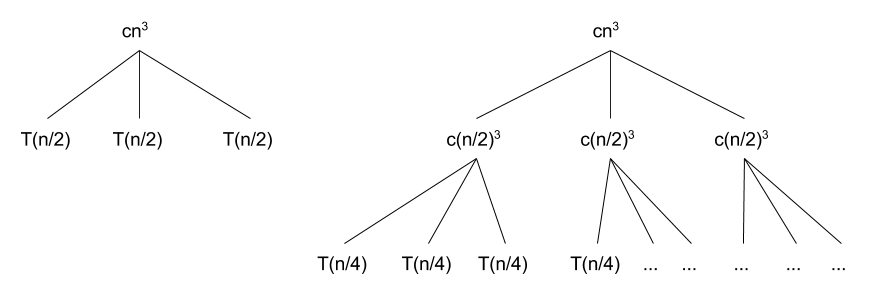
\includegraphics[scale=0.5]{images/rekurrenstre}
\centering %centering the image
\caption{Rekurrenstre}
\label{fig:rekurrenstre}
\end{figure}

\noindent Se Cormen side 64.
\end{boxed}

\subsubsection{Master-metoden}
Selve kokebokmetoden. Hvis du har en rekurrensligning på formen:
\begin{center}
$T(n) = aT(n/b) + f(n)$
\end{center}
\noindent Hvor $a \geq 1$ og $b > 1$ er konstanter og $f(n)$ er en asymptotisk, positiv funksjon, så er det bare å bruke masterteoremt rett fram. Se side 73 i Cormen. I korte trekk sier den at om du lar $n/b$ bety enten $\lfloor n/b \rfloor$ eller $\lceil n/b \rceil$ så har du:

\begin{enumerate}
    \item Hvis $f(n) = O(n^{log_b a-\epsilon})$ for en konstant $\epsilon > 0$, \Rightarrow $T(n) = \theta(n^{log_b a})$
    \item Hvis $f(n) = \theta(n^{log_b a})$, \Rightarrow $T(n) = \theta(n^{log_b a} * log(n))$
    \item Hvis $f(n) = \Omega(n^{log_b a+\epsilon})$ og hvis $a f (n/b) \leq c f (n)$ for en konstant $c > 1$ og $n$ stor nok, \Rightarrow $T(n) = \theta(f(n))$
\end{enumerate}

\begin{boxed}
Anta at du har:
\begin{center}
$T(n) = 9T(n/3) + n$
\end{center}
\noindent Her er $a = 9$, $b = 3$ og $f(n) = n$. Vi ser at:
\begin{center}
$n^{log_3 9} = n^2 = \theta(n^2)$
\end{center}
\noindent Siden $f(n) = O(n^{log_3 9-\epsilon}$ med $\epsilon = 1$, så gir første del av masterteoremet at $T(n) = \theta(n^2)$.
\end{boxed}

\newpage
\section{Rekursjon}
Rekursjon går ut på å bruke samme funksjon flere ganger, med et subset av opprinnelig input. De fleste algoritmer kan implementeres enter iterativt (et funksjonskall som løser problemet), eller rekursivt. Et godt eksempel på dette er fakultet. 

\subsection{Masterteoremet}
Motivasjonen for å lære seg masterteoremet er for å enkelt kunne løse rekurrenser. Ta for eksempel analysen av Mergesort. Hvis vi antar at den originale listen inneholder en 2’er-potens antall elementer vil vi for hvert kall til Mergesort få to nye metodekall med halve listen i hver, helt til antall elementer i listen er lik en. Det vil si at $T(n) = 2T(n/2)$ så lenge $|n| > 1$. 
\\\\
Hovedregelen: $T(N) = aT(n/b) + f(n)$   $a1\geq$, $b \geq 1$
\\\\
Denne typen rekurrenser oppstår gjerne i sammenheng med splitt-og-hersk algoritmer, f.eks. MERGE-SORT. Problemet deles opp i a deler av størrelse $n/b$, med $f(n)$ arbeid for å gjøre selve oppdelingen, og å sette sammen resultatet av rekursive kall etter at disse er ferdige. I eksempelet med MERGE-SORT er $f(n)$ arbeidet med å splitte listen i to underlisten, og å flette sammen de to sorterte listene etter at de rekursive kallene er ferdige. Det å splitte skjer i konstant tid $\theta(1)$, mens det å flette tar lineær tid $\theta(n)$. Vi kan altså sette $f(n) = n$. Siden vi til enhver tid deler listen opp i to deler, hver del $n/2$ er henholdsvis $a = 2$ og $b = 2$. For MERGE-SORT har vi altså: $T(n) = 2T(n/2) + n$
\\\\
Dersom vi ikke allerede visste kjøretiden til MERGE-SORT kunne vi funnet den ved å løse denne rekurrensen. Å løse rekurrensen kunne vi så brukt Masterteoremet til. Fremgangsmåten for Masterteoremet er som følger:
\begin{enumerate}
    \item Identifiser $a$, $b$, $f(n)$
    \item Regn ut $log_b a$
    \item Konsulter tabellen \ref{tab:masterteoremet}
\end{enumerate}

\begin{table}[H]
    \caption{De tre tilfellene av masterteoremet}
    \label{tab:masterteoremet}
    \centering
    \begin{tabular}{|L{5em} | L{18em}|L{18em}|}
        \hline
        \rowcolor[HTML]{303F9F}
        \textbf{\textcolor{white}{Tilfelle}} & \textbf{\textcolor{white}{Krav}} & \textbf{\textcolor{white}{Løsning}}\\
        \rowcolor[HTML]{E6E6E6}
        1 & $f(n) \in O(n^{log_b a-\varepsilon})$ & $T(n) \in \theta(n^{log_b a})$ \\
        2 & $f(n) \in \theta(n^{log_b a} log^k n)$ & $T(n) \in \theta(n^{log_b a} log^{k + 1}n)$ \\
        \rowcolor[HTML]{E6E6E6}
        3 & $f(n) \in \Omega(n^{log_b a+\varepsilon})$ & $T(n) \in \theta(n)$ \\
         \hline
    \end{tabular}
\end{table}

\subsubsection{Eksempel}
\newpage
\section{Sortering og søking}
\subsection{Sortering}
\subsubsection{Stabilitet}
\subsubsection{Sammenligningsbaserte sorteringsalgoritmer}
\large{Merge sort}\\
\large{Quicksort}\\
\large{Bubblesort}\\
\large{Insertion sort}\\
\large{Selection sort}\\
\subsubsection{Andre sorteringsalgoritmer}
\large{Heapsort}\\
\large{Counting sort}\\
\large{Radix sort}\\
\large{Bucketsort}\\
\subsection{Søking}
\subsubsection{Brute force}
\subsubsection{Binærsøk}
\newpage
\section{Grafer og grafalgoritmer}
Ofte har vi ikke bare ett sett med elementer som skal behandles men også forbindelser mellom disse. Dette kan representeres ved hjelp av en graf.
\\\\
En graf, $G = (V,E)$, består av noder (V for \textit{vertices}) og kanter (E for \textit{edges}). Begge deler kan inneholde informasjon. For eksempel kan nodene være hus og kantene være veier mellom husene. Veiene kan ha ulik lengde eller andre egenskaper som gjør at hvilken vei vi velger ikke er avhengig av hvor mange hus vi må innom. Vi sier at kantene har forskjellige kostnader. Dessuten kan veiene være enveiskjørte.

\begin{itemize}
    \item \textbf{Naboer:} To noder er \textit{naboer} dersom det går en kant mellom dem. Nabonoder sies å være \textit{adjacent}.
    \item \textbf{Rettet:} Vi har en \textit{rettet graf} (\textit{firected path}) dersom kantene har retning og kun kan brukes den ene veien (piler).
    \item \textbf{Urettet:} En graf er \textit{urettet} (\textit{undirected}) dersom kantene ikke har noen spesiell retning og kan brukes begge veier.
    \item \textbf{Sykel:} Vi har en \textit{sykel} i en rettet graf dersom det enten finnes en kant som går fra en node og tilbake til samme node, eller vi kan gå fra en node, gå innom noen andre noder og til slutt komme tilbake til den samme noden igjen (ved bare å bevege seg i pilens retning). En graf er \textit{syklisk} dersom den inneholder sykler. I en urettet graf gjelder det samme, men for at det skal regnes som en sykel må vi her passe på å ikke bruke noen kanter begge veier.
    \item \textbf{Vektet:} Vi har en \textit{vektet graf} dersom kantene har forskjellige \textit{vekter} eller \textit{kostnader}. 
    \item \textbf{$k$-fargbar:} En graf er \textit{k-fargbar} dersom man ved hjelp av maksimal \textit{k} i forskjellige farger kan fargelegge nodene (én farge per node) uten at to nabonoder får samme farge.
    \item \textbf{DAG (Directed Acyclic Graph):} En rettet graf som ikke inneholder noen sykler. Disse kan sorteres topologisk. Rettede trær er spesialtilfeller av DAGer.
    \item \textbf{Komplett:} En urettet graf er \textit{komplett} dersom alle nodene er forbundet med hverandre.
    \item \textbf{Kritisk punkt/bro:} En node er et \textit{kritisk punkt} (\textit{articulation point}) dersom fjerning av denne noden vil etterlate en ikke-sammenhengende graf.
    \item \textbf{Bro:} En kant er en \textit{bro} dersom fjerning av denne kanten vil etterlate en ikke-sammenhengende graf.
    \item \textbf{Sti:} En \textit{sti} (\textit{path}) er en vei gjennom grafen eller deler av den. En \textbf{enkel sti} (\textit{simple path}) er en vei som er innom hver node maks en gang. To noder er forbundet (\textit{connected}) hvis det går en sti mellom dem.
    \item \textbf{Hamiltonsti/-sykel:} Nodene besøkes én og bare én gang langs en sammenhengende vei gjennom grafen (langs kantene). Dvs.: vi har en enkel sykel gjennom alle nodene i grafen.
    \item \textbf{Euler-sti:} Kantene benyttes en og bare en gang når vi traverserer/går gjennom grafen (uen å hoppe). Euler viste at en slik sti bare finnes dersom vi har 0 eller 2 noder med odde antall naboer.
\end{itemize}

\subsection{Implementasjon}
En graf kan implementeres på flere måter. Det vanligste er å implementere den som en \textbf{nabomatrise}. Vi setter altså 1 i matrise [a][b] dersom det går en kant fra a til b, og ellers nuller. Legg merke til at dersom vi jar en urettet graf, trenger vi egentlig bare halve matrisen, men det er mye enklere å ha en hel, kvadratisk matrise, som vi passer på at er symmetrisk. Dersom grafen er vektet, fyller vi ut matrisen med kantvektene i stedet, og setter inn $\infty$ der hvor det ikke finnes kanter.

\begin{figure}[H]
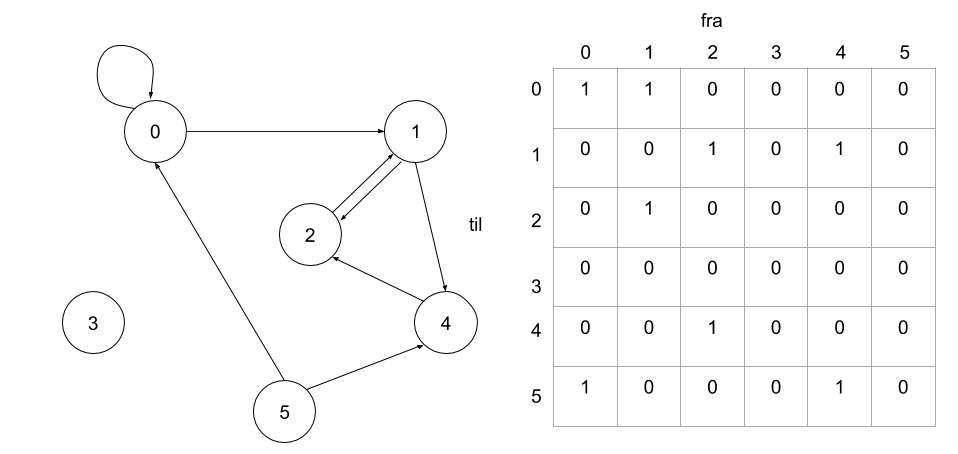
\includegraphics[scale=0.5]{images/implementasjon}
\centering %centering the image
\caption{Implementasjon}
\label{fig:implementasjon}
\end{figure}

\noindent Det finnes flere måter å implementere grafen på; for eksempel kan den representeres som en array av lenkede lister, hvor listen på posisjon \textit{i} forteller hvilke noder som er naboene til node \textit{i}.

\subsection{Representasjon}
\subsubsection{Nabolister}
\subsubsection{Nabomatriser}
\subsection{Traversering}
Her skal vi gjennom to måter å gå systematisk gjennom er graf på. Disse metodene er det veldig vitkig å kunne og forstå.

\subsubsection{Dybde-først-søk (DFS)}
Prinsippet er at grafen skal utforskes i dybden. Det betyr at den neste kanten du skal utforske, går fra den noden du sist oppdaget. Dersom denne noden ikke har noen kanter som går til noder du ikke har oppdaget før, går du tilbake til forrige node og gjør det samme der, osv. Kort fortalt går du utover i grafen så langt du kommer før du trekker deg tilbake og går framover igjen så snart du får muligheten til det.
\\\\
Dette prinsippet kan illustreres ed hjelp av en stakk (LIFO). Den noden som ligger på toppen er den neste som skal utforskes. Hvis denne har en kant til en annen node som vi ikke har truffer på før, legges denne nye noden øverst. Hvis den noden som ligger på toppen ikke har noen kanter til en uutforsket node, tas noden ut av stakken og legges i en liste over ferdighbehandlede noder. Ofte er det nok å bare holde rede på om hver node er truffet på eller ikke, men i noen sammenhenger ønsker man å ha en trefarging av nodene: uoppdagede noder er hvite, noder som er oppdaget og fortsatt ligger i stakken er grå, og ferdigbehandlede noder er svarte. Se kapittel 22.3 i Cormen.
\\\\
Legg merke til at dersom det går flere kanter ut fra den noden du skal undersøke til andre uoppdagede noder, spiller det i prinsippet ingen rolle hvilken du velger. Forskjellige valg vil gi forskjellige resultater, men alle vil være gyldige. Når duskal implementere DFS, er det imidlertid greit å bestemme seg for en eller annen regel, for eksempel at naboene skal behandles i alfabetisk rekkefølge, eller i den rekkefølgen de er oppgitt i nabolisten. Merk at hvis noden øverst på stacken, la oss si node \textit{X}, har flere naboer, så skal \textit{ikke} alle slenges inn i stakken på en gang; først skal en av dem, f.eks. node \textit{Y}, legges inn, og så jobber man videre med den. Ikke før node Y er ferdigbehandlet og fjernet fra stacken (og node \textit{X} således dukker opp på toppen igjen) skal man gå videre med neste nabo (hvis denne naboen fremdeles er ubesøkt – det kan jo hende at søket fra node \textit{Y} fant frem hit).
\\\\
Når stacken er tom er du i utgangspunktet ferdig, men der er ikke sikkert ar du nådde ut til hele grafen fra den noden du startet på, for det er ikke alltid det er forbindelse mellom alle nodene i en graf. Dersom du er interessert i å utforske \textit{hele} grafen med DFS må du, hver gang stacken er tom, sjekke om alle nodene er blitt besøkt. Dersom det er flere uoppdagede igjen, dytter du en av dem inn i stacken og starter et nytt DFS derfra. Dette gjentar du til alle nodene er oppdaget.

\begin{boxed}
Vi oppretter stakken "oppdaget", hvor vi legger nodene etterhvert som vi oppdager dem, og listen "ferdig", hvor vi legger de ferdig utforskede nodene.\newline\newline
Vi begynner på A og traverserer grafen etter prinsippene over. Følg med på hvordan vi beveger oss i grafen.

\begin{figure}[H]
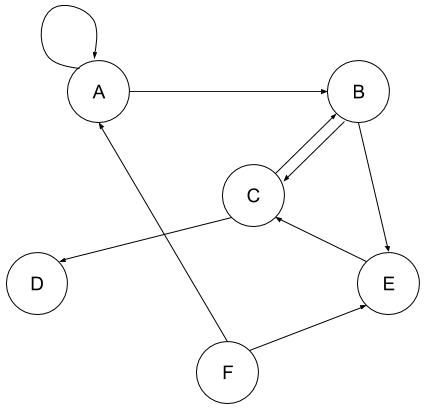
\includegraphics[scale=0.5]{images/DFS}
\centering %centering the image
\caption{Traversering av DFS}
\label{fig:DFS}
\end{figure}

1. oppdaget: A; ferdig: - (A har seg selv som nabo, men A er jo oppdaget, så vi tar B i stedet)\\\\
2. oppdaget: A, B; ferdig: - (B har to naboer, C og E, og vi velger å fortsette med C – men det hadde også vært tillatt å fortsette med E)\\\\
3. oppdaget: A, B, C; ferdig: - (C har B som nabo, men B er oppdaget, så vi tar D i stedet)\\\\
4. oppdaget: A, B, C, D; ferdig: - (D har ingen naboer, så vi er ferdig med D og kan fjerne den fra stacken)\\\\
5. oppdaget: A, B, C; ferdig: D (vi er nå tilbake på C, som ikke har flere ubesøkte naboer, så vi er ferdige med den også)\\\\
6. oppdaget: A, B; ferdig: D, C (B har E som ubesøkt nabo)\\\\
7. oppdaget: A, B, E; ferdig: D, C (E har ingen ubesøkte naboer)\\\\
8. oppdaget: A, B; ferdig: D, C, E (osv.)\\\\
9. oppdaget: A; ferdig: D, C, E, B\\\\
10. oppdaget: -; ferdig: D, C, E, B, A (stakken er tom, så nå går vi gjennom alle nodene og ser etter ubesøkte noder – det viser seg at F er ubesøkt, så vi legger inn den)\\\\
11. oppdaget: F; ferdig: D, C, E, B, A (F har ingen ubesøkte naboer)\\\\
12. oppdaget: -; ferdig: D, C, E, B, A, F (stakken er tom og det er ingen ubesøkte noder igjen; vi er ferdige)
\end{boxed}

\begin{lstlisting}
    function DFS(G,v)	//v er startnode
	    initialiser en tom stack, S
    	for each vertex u in G do
    		set visited[u] $\rightarrow$ false
    	end for
    	S.push(v)
    	while S.notEmpty() do
    		u = S.pop()
    		for all w adjacent to u do
    			if not visited[w] then
    				visited[w] $\rightarrow$ true
    				S.push(w)
    			end if
    		end for
    	end while
    end function
\end{lstlisting}

\subsubsection{Bredde-først-søk (BFS)}
Prinsippet er at grafen skal utforskes i bredden. Det betyr at du utforsker alle kantene ut i fra den noden du står i før du beveger deg til neste node. 
\\\\
Dette prinsippet kan illustreres ved hjelp av en kø (FIFO). Den noden som ligger først i køen, la oss kalle den \textit{X}, er den vi skal utforske naboene til. De ubesøkte nodene som \textit{X} har kanter til legges bakerst i køen (rekkefølgen spiller i prinsippet ikke noen rolle her). Deretter fjernes \textit{X} fra køen og legges i en liste med ferdigbehandlede noder.
\\\\
Også her er det mulig at alle nodene ikke er forbundet, men når man bruker BFS, er man som regel kun interessert i nodene som kan nås fra den opprinnelige startnoden. Derfor gir man seg med en gang køen er blitt tom, uten å sjekke om det finnes uoppdagede noder.
\\\\
BFS egner seg godt til å finne ut hvor mange kanter som er nødvendig å bruke for å komme seg fra startnoden til de andre nodene. Grunnen til dette er at det første vi gjør, er å se på alle naboene til startnoden – disse ligger jo 1 kant unna. Deretter vil hver av disse nodene plukkes ut av køen, og alle de ubesøkte naboene deres må nødvendigvis ligge 2 kanter unna startnoden osv. Når vi tar ut en node fra køen kan vi dermed markere alle de ubesøkte naboene dens med en avstand på 1 mer enn nodens egen avstand. Startnoden har naturlig nok avstand 0 til seg selv.

\begin{boxed}
Vi oppretter køen "oppdaget", hvor vi legger nodene etterhvert som vi oppdager dem, og listen "ferdig" hvor vi legger de ferdigbehandlede nodene.

\begin{figure}[H]
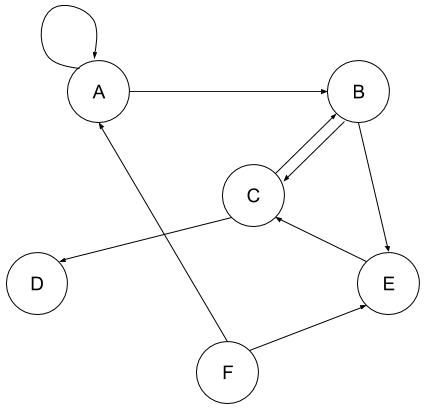
\includegraphics[scale=0.5]{images/DFS}
\centering %centering the image
\caption{Traversering av BFS}
\label{fig:BFS}
\end{figure}
1. oppdaget: A(0); ferdig: - (A sine naboer er A og B, men A er jo allerede oppdaget, så kun B vil legges inn, og avstanden vil bli 1)\\\\
2. oppdaget: B(1); ferdig: A(0) (B sine to naboer er C og E vil legges inn med avstand 2)\\\\
3. oppdaget: C(2); ferdig: A(0), B(1)\\\\
4. oppdaget: E(2), D(3); ferdig: A(0), B(1), C(2) (E har ingen ubesøkte naboer)\\\\
5. oppdaget: D(3); ferdig: A(0), B(1), C(2), E(2)\\\\
6. oppdaget: -; ferdig: A(0), B(1), C(2), E(2), D(3) (Køen er nå tom, og vi er ferdige – F ble ikke besøkt fordi den ikke kunne nås fra A)\\\\
Legg merke til hvordan nodene kommer ut av køen i stigende rekkefølge med hensyn på avstand fra startnoden.
\end{boxed}

BFS implementeres med en kø. BFS utforsker grafen i bredden. Man starter på foreldrenoden og legger inn alle dens barn i køen. Når alle naboer til node $x$ er oppdaget, fjernes den fra køen og man tar den neste noden i køen og legger alle dens barn inn i køen. Når køen er tom, sjekker man ikke videre om det er ubesøkte noder.

\begin{lstlisting}
    function BFS(G,v) // v er startnode
	    lag en kø Q
    	legg v inn i Q
    	while Q.notEmpty() do
    		v = Q.dequeue()
    		for each edge e adjacent to v do
    			if e not marked then
    				mark w
    				Q.enqueue(e)
    			end if
    		end for
    	end while
    end function

\end{lstlisting}


\noindent \textbf{Traversering}

\subsection{Korteste vei}
Denne typen problemer er ekstremt nyttig i mange sammenhenger. Hvis man skal kjøre bil fra et sted til et annet, vil man gjerne kjøre den korteste veien for å spare bensin og tid. I dette tilfellet holder det å se på veilengden som en kostnad for hver kant. I dette tilfellet blir kostnaden alltid positiv, men det trenger den ikke bli i andre eksempler. Hvis man skal dra rundt og selge ting og er ute etter å se på hvor mye man tjener på forskjellige ruter, kan det hende man vet at det på enkelte strekninger vil bli tap. Men det er fortsatt mulig å finne ut hvilken vei det lønner seg å ta for å tjene mest mulig penger.

\subsubsection{Én til alle}
Her vi vil konsentrere oss om de problemene som har ett startpunkt, og som går til alle tenkelige sluttpunkt i den mengden man ser på. Anta at vi er fire studenter som deler kjøkken på Nedre Singsakerslette, og alle har sin egen bil og skal hjem til jul. Førstemann bor i Drøbak, den andre på Kolbotn, nummer tre på Tretten, og fjerdemann i Malvik. Da holder det at man kjører en algoritme for korteste vei, én-til-alle-problem (her kan man også benytte seg av det gunstige faktum at alle kostnader er positive, noe som dere etterhvert vil se gir enklere og raskere algoritme). Med et kart over alle byer og veier i Norge er det bare å bruke Trondheim som startpunkt og kjøre en algoritme for å finne de korteste veiene fra Trondheim til alle de andre byene, og så sjekke rutene man fikk til Drøbak, Kolbotn, Tretten og Malvik. Dermed kan alle ta hver sin bil (ikke så veldig sosialt eller økonomisk, men eksempelets intensjon helliger midlet) og kjøre korteste vei til sin hjemby. 
\\\\
Et viktig prinsipp i alle korteste-vei-problemene, er det som kalles \textbf{relaxation}. Dette er ikke noe mer skummelt enn at man sjekker en eller annen kant fra en node \textit{u} til en annen node \textit{v}, og skulle denne kanten tilby en kortere vei til \textit{v} enn den veien vi eventuelt hadde fra før, oppdaterer man node \textit{v} med informasjon om at den korteste veien nå kommer fra node \textit{u}. Skulle den veien man prøver være lenger, oppdaterer man ikke.

\begin{figure}[H]
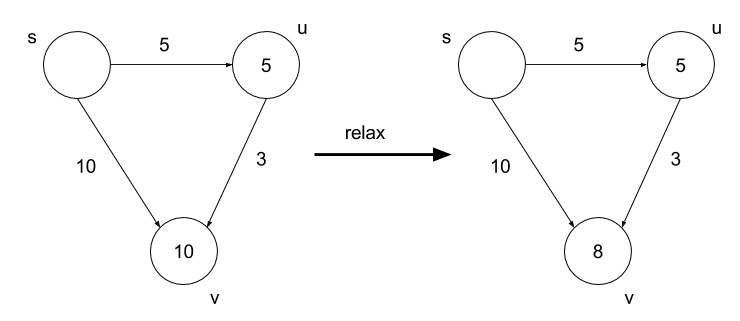
\includegraphics[scale=0.5]{images/relaxation}
\centering %centering the image
\caption{Relaxation. Tallet i noden angir funnet avstand fra kilden.}
\label{fig:relaxation}
\end{figure}

\noindent En viktig ting å ha i mente, er at korteste vei \textbf{ikke kan ha sykler}. Har man en \textbf{positiv sykel}, så vil man ved å fjerne denne sykelen fortsatt ha en vei mellom sine to noder som også blir kortere enn om man brukte sykelen. Har man en sykel med verdi 0, så blir denne helt uniteressant, og man kan like godt droppe den. Hvis det eksisterer en \textbf{negativ sykel}, så vil man kunne gå rundt denne negative sykelen så mange ganger man vil og få stadig kortere vei. Dermed vil det ikke kunne være en bestemt korteste vei, da man alltid kan ta en ny runde i den negative syklen og få en enda kortere vei. Negative sykler ødelegger faktisk hele problemstillingen, og ingen av algoritmene våre vil klare å finne noe godt svar dersom grafen inneholder en negativ sykel som kan nås fra startnoden. Merk dog at en graf kan inneholde negative kanter uten å ha negative sykler.\\

\noindent\textbf{Bellman-ford}\\
Denne algoritmen tar for seg de problem hvor kostnadene på kantene til grafen kan være negative. Dermed blir den ganske generell. Hvis det eksisterer negative sykler, returnerer Bellman-Ford "FALSE". Men om slike negative sykler ikke forekommer (vel og merke holder det at de ikke kan nås fra utgangspunktet vårt), så returnerer algoritmen beste vei.
\\\\
Algorimen fungerer som følger (se også s. 588 i Cormen):
\begin{enumerate}
    \item La antall noder i grafen være \textit{|V|}. Følgende gjøres \textit{|V| - 1} ganger: Gå gjennom alle kantene og kjør \textit{relax} på hver av dem. Når man er ferdig med dette, vil man faktisk ha funnet den korteste veien (vel og merke om man ikke har en negativ sykel). Studér kommende eksempel, og prøv å forstå hvorfor det må bli slik – ta gjerne \textit{path-relaxation property} fra side 587 i Cormen til hjelp (den sier at hvis kantene på den korteste veien mellom to  noder blir "relaxed" i riktig rekkefølge, selv hvis det foregår mange andre relaxations imellom, vil man få en riktig verdi for korteste avstand). Alle veier mellom nodene vil være utprøvd, og den korteste veien blir funnet takket være path relaxation property.
    \item Deretter gjelder det å finne ut om vi faktisk har en negativ sykel. Dette gjør man ved å sjekke samtlige kanter i grafen. La oss si at vi har en kant fra node \textit{u} til node \textit{v}, kann denne kanten (\textit{u,v}). Hvis summen av kostnaden fra startnoden til node \textit{u} og kostnaden til (\textit{u,v}) blir mindre enn verdien vi fant for kostnaden fra startnoden til \textit{v}, vil dette bety at man har en negativ sykel. Dette bevises i Cormen på side 590.
\end{enumerate}

\noindent Hvis man kaller antallet noder for \textit{|V|} og antallet kanter for \textit{|E|}, blir kjøretiden til Bellman-Ford-algoritmen ganske enkelt $O(|V||E|)$. Dette ser man lett, da man går gjennom alle nodene en gang for hver gang man tar for seg en node vil man måtte sjekke et antall kanter som er proposjonalt med antallet kanter som eksisterer. For å sjekke negative sykler tar det bare $\theta(|E|)$ i tid, så denne vil ikke påvirke den asymptotiske kjøretiden fra første del av algoritmen.

\begin{figure}[H]
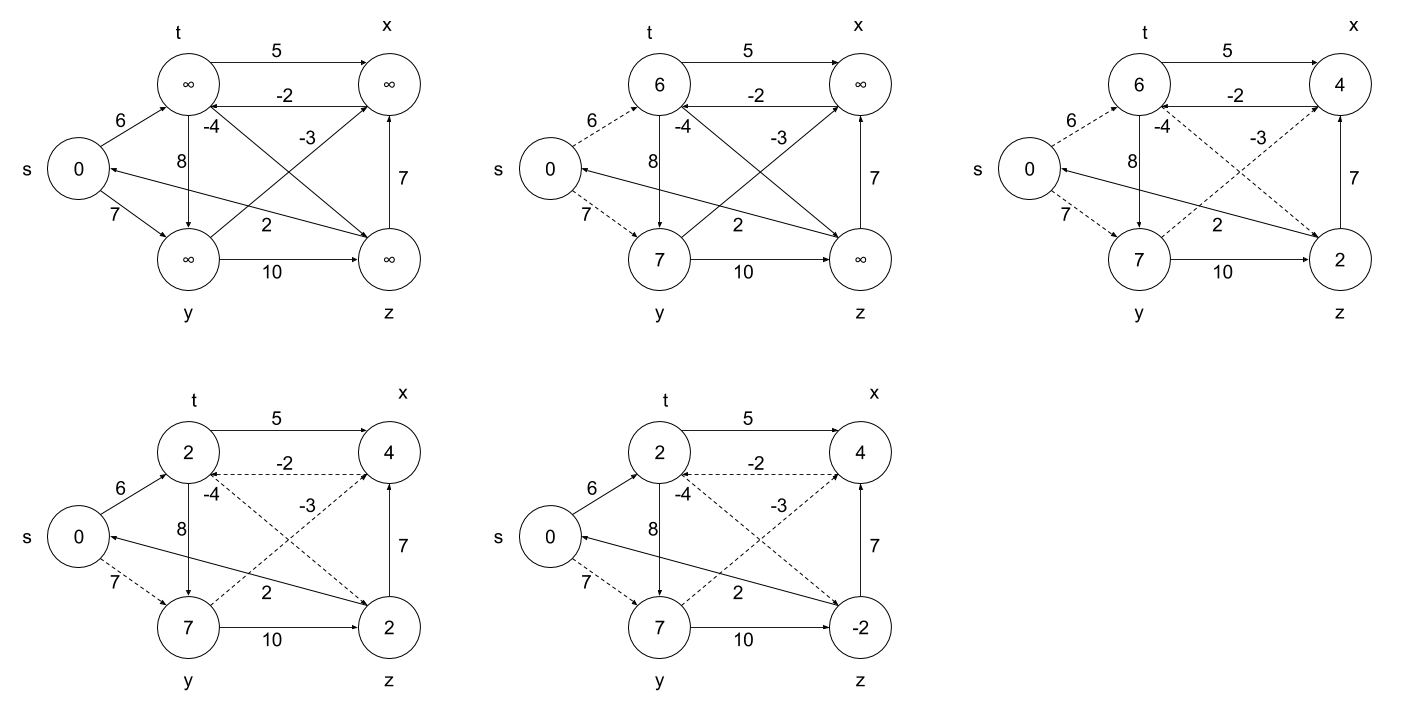
\includegraphics[scale=0.3]{images/bellman-ford}
\centering %centering the image
\caption{Bellman-Ford}
\label{fig:bellman-ford}
\end{figure}

\noindent\textbf{Dijkstras algoritme}\\
Kravet for å bruke Dijkstras algoritme er at alle kantene har positive verdier (eventuelt også verdien 0). Da kan man bruke en smartere algoritme enn Bellmann-Ford. Dijkstrra er faktisk en \textbf{grådighetsalgoritme}. Pseudokode står på side 595 i Cormen.
\\\\
Dijkstra er en korteste vei, en-til-alle-algoritme. Tillater ikke negative kanter. Den velger noder en etter en fra hvor nærme de er startnoden. 
\\\\
Det faktum at grågighetsprinsippet fungerer her, gjør at man kan kjøre gjennom en algoritme som ikke tester alt det som Bellmann-Ford måtte ha testet. Hvorfor grådighet vil fungere, er ikke så vanskelig å se for seg. Hvis du bruker 10 liter bensin bort til Ola og 15 liter til Mogens, vil det aldri i verden kunne være lønnsomt å dra via Mogens til Ola hvis vi ser på bensinforbruket. For vi må nødvendigvis svi av noe bensin mellom Ola og Mogens, så uansett hva vi forbruker mellom disse to fyrene vil det fra et bensin-perspektiv være ulønnsomt å dra via Mogens (ja, det finnes selvsagt argumenter for å besøke Mogens. Det kan jo være direkte hyggelig, og dessuten gir han deg kanskje bensin gratis. Men i dette tilfellet vil denne bensinen Mogens gir deg regnes som et negativt forbruk, og vi kan ikke bruke Dijkstra).
\\\\
Kort fortalt plukker Dijkstra ut nodene en etter en ut fra hvor nær de er startnoden hvis vi følger korteste vei. Den første noden som plukkes ut er startnoden (husk at dette er en én-til-alle-algoritme). Deretter kjøres relaxation til alle andre noder for å finne neste node som skal plukkes ut tas ikke med i neste runde med relaxation. Dette gjentas til vi har funnet korteste vei til alle nodene. 

\begin{boxed}
En gjeng syklister er samlet på startstreken (startnoden) til et sykkelritt. Alle er like spreke og sykler nøyaktig like fort hele tiden. Vi lar kostnaden mellom to noder være tiden det tar for en syklist å sykle fra den ene til den andre. Målet i et tradisjonelt sykkelritt er selvsagt å komme først i mål, men her er det snakk om å finne korteste vei til alle nodene.\newline\newline
Det er mange veilvalg underveis, men vi antar at det er så mange syklister at det alltid er minst en til hvert veivalg. Slik vil den eller de syklisten(e) som besøker en node først, ha funnet den korteste veien til denne noden og tiden han/de brukte illustrerer kostnaden til denne veien.
\newline\newline
Det er akkurat slik Dijkstra finner de korteste veiene; så fort en syklist når fram til en hittil ubesøkt node, legges den til i mengden med noder vi har funnet kortest vei til.
\end{boxed}

\begin{figure}[H]
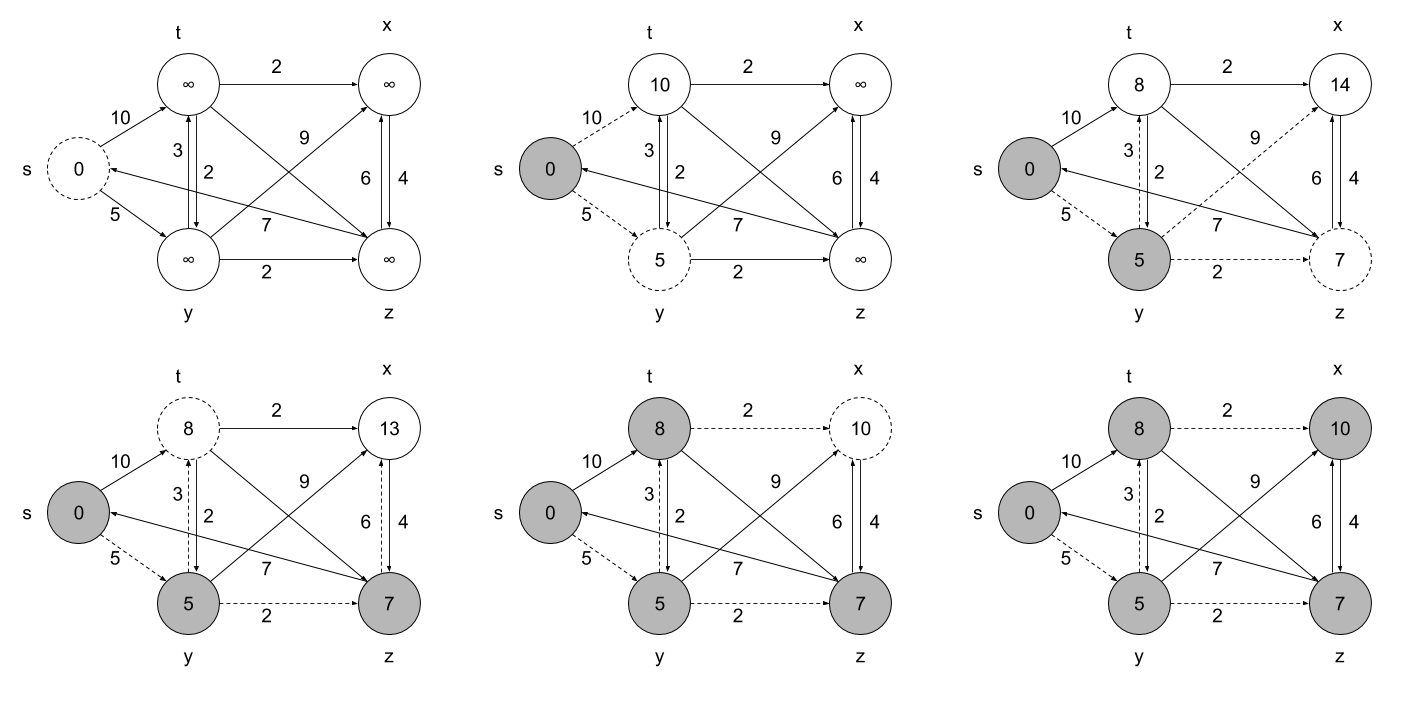
\includegraphics[scale=0.3]{images/dijstra}
\centering %centering the image
\caption{Dijkstra}
\label{fig:dijkstra}
\end{figure}

\noindent Det kan vises at kjøretiden til Dijkstra er $O(|V|^2)$ i de fleste tilfeller, men den kan gjøres bedre om man har god kunnskap om grafen man ser på. Merk at $O(|V|^2)$ er bedre enn $O(|V||E|)$, fordi antallet kanter $|E|$ minst må være $|V| - 1$ mens den øvre grensen faktisk kan være asymptotisk med $|V|^2$.

\begin{lstlisting}
    function DIJKSTRA(G,w,s)
	    INITIALIZE-SINGLE-SOURCE(G,s)
    	S = Ø
    	Q = G.V
    	while Q $\neq$ Ø do
    		u = EXTRACT-MIN(Q)
    		S = S $\cup$ {u}
    		for each vertex v $\in$ G.Adj[u] do
    			RELAX(u,v,w)
    		end for
    	end while
    end function
\end{lstlisting}

\noindent Hvis man har en DAG, vil det ikke oppstå noen vanskeligheter selv om man har negative kostnader på kantene, for i en DAG vil det ikke eksistere noen sykler i alle tilfeller. Trikset for å finne korteste vei er i første rekke å gjøre en topologisk sortering av DAGen. Slik oppnår vi en lineær ordning av nodene. Deretter trenger vi bare besøke nodene en gang i den topologisk sorterte rekkefølgen og kjøre en relaxation for hver gang til de noder som ligger foran. 
\\\\
Kjøretiden vil avhenge av den topologiske sorteringen, og en slik sortering har kjøretid $\theta(|V|+|E|)$. Ingen andre ledd i algoritmen for korteste vei i en DAG vil bli større enn den topologiske sorteringen, så kjøretiden blir $\theta(|V|+|E|)$.\\

\noindent\textbf{DAG shortest path}\\
DAG-Shortest-Path er en korteste vei, en-til-alle algoritme. Tillater ikke negative kanter, og kan selvfølgelig ikke ha sykler, da det er en DAG. Gjør topologisk sortering av DAGen og besøker hver node en gang for å kjøre RELAX på nodene foran.

\begin{lstlisting}
    function DAG-SHORTEST-PATH(G,w,s)
    	TOPOLOGICAL-SORT(G)
    	INITIALIZE-SINGLE-SOURCE(G,s)
    	for each vertex u, taken in topologically sorted order do
    		for each vertex v ∈ G.Adj[u] do
    			RELAX(u,v,w)
    		end for
    	end for
    end function

\end{lstlisting}

\subsubsection{Alle til alle}
En soleklar måte å takle dette problemet på, er rett og slett å bruke en god algortime for et én-til-alle-problem, og så bruke denne på samtlige noder som startnoder. Dette er ikke så dumt som det kan høres ut som. Hvis alle kostnadene er ikke-negative, fungerer det meget bra å bruke Dijkstra. Kjøretiden her vil bli $O(|V|^3)$, som man ser ved å multiplisere kjøretiden til en gjennomgang av Dijkstra med antallet noder $|V|$. Hvis vi har negative kostnader og kjører samme trikset med Bellman-Ford, blir kjøretiden $O(|V|^2 |E|)$, som ikke er så veldig bra fordi $|E|$ er av størrelsesorden $|V|^2$. Nå skal det sies at med meget smarte fremgangsmåter her, vil disse kjøretidene kunne senkes betraktelig. Men vi bruker heller en algoritme som tar for seg problemet med alle-til-alle uten å skulle gå omveien om mange gjennomkjøringer av en én-til-alle-algoritme.\\

\noindent\textbf{Floyd-Warshall}\\
Ved å benytte oss av prinsippet om \textbf{dynamisk programmering} skal vi her vise hvordan Floyd-Warshall-algoritmen fungerer.
\\\\
Pseudokoden for Floyd-Warshall er relativt grei. Man lager en nabomatrise til nodene, men gjør litt om på den. Hvis det går en vei fra en node til en annen, setter vi verdien til å være kostnaden på kanten mellom dem. Går det ikke en direkte kant mellom de to nodene, settes kostnaden til å være uendelig ($\infty$). Deretter velger man seg en node, kall noden \textit{a}, som man har lov til å gå innom. Så tester man veien mellom to og to noder, kall dem \textit{u} og \textit{v}. Hvis det koster mindre å gå via \textit{a}, så legger man inn denne veien til å være den korteste. Nå har vi en oversikt over de korteste veiene som kun består av enkeltkanter eller som bruker node \textit{a} (og ingen andre). Så kan vi gå videre og tillate en annen node, \textit{b}, og sjekke om vi kan få kortere veier ved å ta den i bruk osv. Etter å ha gått gjennom alle nodene på denne måten vil vi til slutt ha en oversikt over de korteste veiene uten noen begrensninger på hvilke noder som kan brukes. Det er heller ikke så veldig vanskelig å lage enda en nabomatrise som holder styr på hvilke noder man skal gå innom for å oppnå denne ultimate veien. Det er ikke så rent ulogisk at dette vil fungere, men det gjelder å få et godt grep om hva som skjer.


\begin{figure}[H]
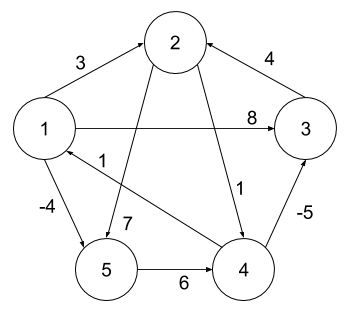
\includegraphics[scale=0.5]{images/floyd-warshall}
\centering %centering the image
\caption{Floyd-Warshall. Tallene i noden betyr her nummeret på noden, ikke avstand.}
\label{fig:floyd-warshall}
\end{figure}

\noindent Figuren viser grafen til problemet vårt. Om vi bruker algoritmen på siden 630 i Cormen, vil matrisene under utregning bli slik du ser under her. Merk at indeksen i hver matrise betyr hvilken node vi har gått innom. Den første, med indeks 0, er startmatrisen. 
\\\\
\noindent Kjøretiden til Floyd-Warshall er ganske enkelt $O(|V|^3)$. Det er $|V|$ noder man skal innom, og for hver gang kan man variere startnoden med $|V| - 1$ muligheter og sluttnoden med $|V| - 2$ muligheter. Om man ser på pseudokoden i Cormen, så ser man at den består av tre greie for-løkker. Nå skal det sies at også Dijkstra på alle nodene gir $O|V|^3$, men operasjonen per ledd i Floyd-Warshall er så mye mindre at denne stort sett vil lønne seg selv hvis alle kantene er positive. Dersom det er relativt få kanter i forhold til noder vil derimot Dijkstra med heap (som kjører på $O(|E| lg |V|)$ for hver av de $|V|$ nodene) lønne seg.

\subsection{Maksimal flyt}
I stedet for å la kostnaden til kanten mellom to noder representere avstand eller pris, som i Floyd-Warshall, så er det i noen situasjoner gunstig å operere med en kapasitet og en flyt mellom nodene. Denne flyten kan være meget generell, så maks-flyt-problemer spenner over et stort område. I et maks-flyt-problem ønsker vi å finne den største flyten fra en gitt kilde til et gitt sluk uten å overskride noen kapasitetskrav.

\subsubsection{Flytnettverk}
Et flytnettverk $G = (V,E)$ (hvor V står for nodene og E for kantene) er en rettet graf hvor hver kant (\textit{u,v}) har en ikke-negativ kapasitet $c(u,v) \geq 0$. Eksisterer det ingen kant mellom to noder, setter vi kapasiteten til å være null. To av nodene er av spesiell betydning. Det er kilden \textit{s}, som er den eneste noden som kan produsere flyt, og sluket \textit{t}, som er den eneste noden som kan ta imot flyt uten å sende den videre. Vi kan nå definere flyt på følgende måte:
\begin{center}
En flyt i G er en funksjon: $f: V * V \rightarrow$  ${\Bbb R}$
\end{center}

\noindent slik at følgende tre krav er oppfylt:
\begin{itemize}
    \item \textbf{Kapasitet:} For alle \textit{u, v} $\in V$ så krever vi $f (u,v) \leq c (u,v)$. Flyten må altså ikke overstige kapasiteten.
    \item \textbf{Symmetri:} For alle $u,v \in V$ så krever vi $f (u,v) = -f(v,u)$. Positiv flyt én vei tilsvarer altså en like stor, negativ flyt motsatt vei (akkurat som når man regner på strøm i elektriske kretser).
    \item \textbf{Bevaring av flyt:} For alle $v \in V - \{s,t\}$ (altså for alle noder \textit{v} unntatt kilden og sluket) krever vi at flyten inn må være like stor som flyten ut, dvs. at det ikke "renner over" i noen noder og at ingen noder kan produsere flyt selv. Det kan formuleres som at summen av flyten inn i \textit{v} må være null:
    \begin{center}
    $\sum\limits_{u \in V} f(u,v) = 0$ 
    \end{center}
\end{itemize}

\noindent Det første kravet sier at vi alltid må respektere kapasiteten. Det andre kravet er egentlig bare en formalitet som gjør det mulig å regne med negativ flyt, som generaliserer teorien en hel del. Hvis jeg sender hundre kroner til din konto, vil de gå en positiv flyt av penger fra meg til deg, mens det går en negativ flyt fra deg til meg. Bevaringsloven til sist sier bare at flyt ikke uten videre kan forsvinne eller oppstå. Dette kan sammenlignes med diverse bevaringslover fra fysikken, som f.eks. energibevaring.
\\\\
Vi sier at $|f|$ er flyten fra kilden til sluket, og dens verdi er rett og slett summen av flyten til alle veiene ut fra kilden, som igjen er det samme som summen av flyten inn i sluket. Mer presist:
\begin{center}
    $|f| = \sum\limits_{u \in V} f(s,v)$ 
    \end{center}
    
\noindent Legg spesielt merke til siste krav, som gir at total flyt i en node må være null. Det som kommer inn blir sendt ut igjen med samme rate, det er ingenting som hoper seg opp. Dette kan sammenlignes med Kirchoffs lover for elektrisk strøm. Ellers er den totale positive flyten definert til å være summen av de positive flytene inn i en node, eller:
\begin{center}
    $\sum\limits_{u \in V, f(u,v)>0} f(u,v) = 0$ 
    \end{center}
    
\noindent Hvis vi har flere kilder og sluk, er det et godt triks å legge til en superkilde og et supersluk, slik at vi oversetter problemet til det vi er vant til. Dette gjøres ved å opprette en ny node med kanter til alle kildene. Sett kapasiteten på disse kantene til uendelig (med mindre du ønsker å sette noen spesielle begrensninger på flyten). Tilsvarende skal alle slukene ha en kant til supersluket. I alle videre utregninger skal du tenke på superkilden/-sluket som eneste kilde/sluk.

\begin{figure}[H]
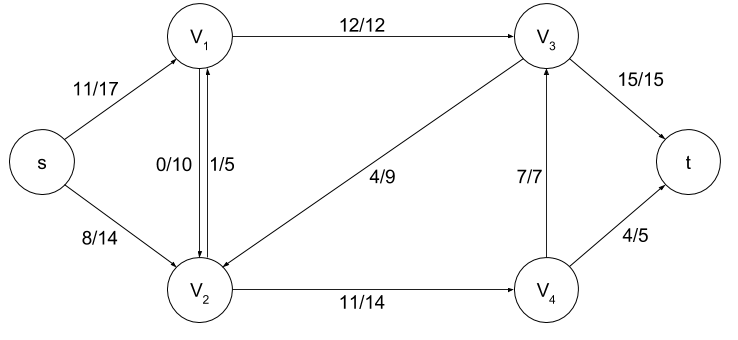
\includegraphics[scale=0.6]{images/flytnettverk}
\centering %centering the image
\caption{Flytnettverk}
\label{fig:flytnettverk}
\end{figure}

\noindent \textbf{Ford-Fulkersons metode}\\
Ford-Fulkerson-metoden er en god algoritme som finner maksimal flyt i et flytnettverk. Hver iterasjon forsøker å finne en flytforøkende sti, og setter på all den flyten som er mulig. Deretter leter den etter en ny flytforøkende sti, og gjentar prosessen. Når det ikke er flere flytforøkende stier har man oppnådd maksimal flyt. Den benytter seg av DFS for å finne flytforøkende sti. Det er altså tre essensielle ideer; residualnettverk, flytforøkende vei, og snitt.\\

\subsubsection{Residualnettverk}
Som uttrykket kanskje tilsier ("residual" betyr "rest"), for et flytnettverk med en gitt flyt, består residual-nettverket av de kantene som tillater mer flyt.

\begin{boxed}
Vi beskriver ofte flyten og kapasiteten ved å skrive en brøk med flyt-verdien øverst og kapasitetsverdien nederst. Man får residual-nettverket ved å ta de opprinnelige kapasiteter og trekke fra den flyten som går i hver kant. Med flyten fra Figur \ref{fig:flytnettverk} får vi residualnettverket til å bli som vist i Figur \ref{fig:residualnettverk.}

\begin{figure}[H]
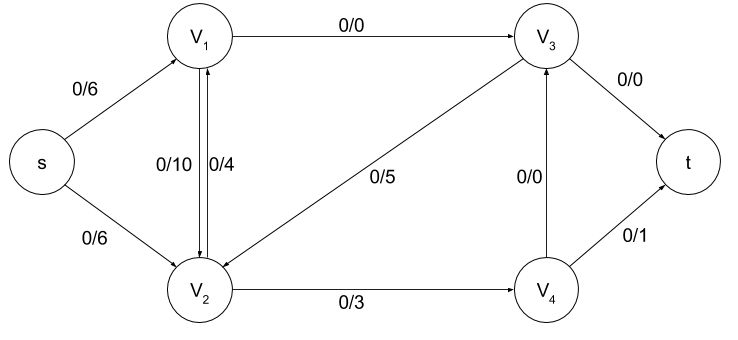
\includegraphics[scale=0.6]{images/residualnettverk}
\centering %centering the image
\caption{Residualnettverk}
\label{fig:residualnettverk}
\end{figure}
\end{boxed}

\subsubsection{Flytforøkende sti}
\subsubsection{Minimalt kutt}
Minimum-snitt (min-cut) på et flytnettverk: det snittet som har lavest kapasitet av alle snitt. Det vil si min-cut angir en flaskehals i flytnettverket. Det vil si at det ikke kan sendes mer flyt gjennom nettverket enn det vi kan sende gjennom flaskehalsen. Man kan da ikke finne noen flytforøkende sti over flaskehalsen. Det vil da være maksimal-flyt, max-flow.\\



\noindent \textbf{Edmonds-Karp}\\
Endret en bokstav på Ford-Fulkerson-metoden. De benytter seg av BFS. Edmonds-Karp bruker Ford-Fulkerson og BFS til å finne flytforøkende stier.\\

\subsection{Topologisk sortering}
La oss si at nodene representerer oppgaver som skal gjøres. Noen oppgaver må gjøres før andre. For eksempel må du lage middagen før du kan spise den. Andre kan gjøres i valgfri rekkefølge. Dette kan illustreres med en rettet graf.
\\\\
Topologisk sortering går ut på å finne en mulig rekkefølge oppgavene kan gjøres og tar utgangspunkt i en DAG. Det er opplagt at topologisk sortering bare har mening når vi har å gjøre med en rettet graf, og den kan ikke inneholde sykler. Dersom vi har sykler eksisterer ingen gyldig løsning.

\begin{boxed}
\begin{figure}[H]
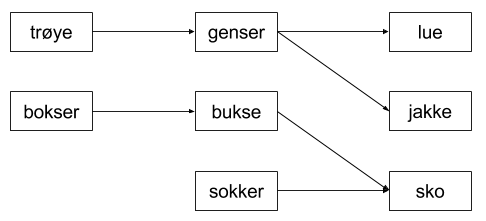
\includegraphics[scale=0.7]{images/topologisk}
\centering %centering the image
\caption{Topologisk sortering}
\label{fig:topologisk}
\end{figure}

Et klassisk eksempel er rekkefølgen du kan kle på deg. I grafen har vi tatt men noen klesplagg, og pilene viser rekkefølgen de må tas på. Det kan selvsagt diskuteres om du må vente med å ta på deg luen til du har tatt på deg genseren, men av erfaring blir det gjerne ekstraarbeid dersom du forsøker annen rekkefølge.
\end{boxed}

\subsubsection{Algoritme}
Topologisk sortering er veldig enkelt når du har forstått DFS. Du kjører rett og slett bare et DFS og lager en liste med oppgavene i den rekkefølgen de fjernes fra stakken. Deretter reverserer du listen, og du vil da ha en gyldig rekkefølge å utføre oppgavene i. Grunnen til at dette virker er at når en node \textit{X} fjernes fra stakken, vet du at du har utforsket alle pilene ut fra \textit{X}, og dermed har vi allerede utforsket de nodene som avhenger av \textit{X} og lagt dem til i listen. Vi kan dermed legge til \textit{X}, og når listen reverseres, vil \textit{X} stå foran alle nodene som avhenger av den.

\begin{boxed}
Vi må begynne traverseringen i en node som ikke har noen piler inn mot seg. Minst én slik node vil finnes, da grafen ikke har noen sykler. Vi kan altså begynne med enten trøye, bokser eller sokker.\newline\newline
Vi velger å begynne med "sokker" (nok en gang er det tillatt å velge fritt blant de aktuelle alternativene). Disse legges øverst i stakken. Vi har bare en vei å gå videre, nemlig til "sko". Ingen piler peker fra "sko", så vi kan være sikre på å ikke besøke noden i grafen igjen, og legger derfor "sko" først i listen \textit{besøktForSisteGang}. Vi går så tilbake til "sokker", og oppdager at heller ikke denne noden kjenner noen noder vi ikke har besøkt enda. "Sokker" legges så til i listen \textit{besøktForSisteGang}. Nå er listen \textit{oppdaget} tom igjen, og vi må søke for å se om det er flere noder i grafen. Det er det, men vi må passe på å velge en som ikke har noen kanter inn mot seg. Vi velger "bokser". Det fører til at "bukse" og "bokser" blir puttet inn i \textit{besøktForSisteGang} i den rekkefølgen. Vi finner så "trøye", går videre til "genser", og velger tilfeldigvis "lue" før "jakke". "Lue" kjenner ingen flere og blir lagt til i \textit{besøktForSisteGang}. Vi går tilbake til "genser", som også kjenner "jakke". "Jakke", "genser" og "trøye" blir lagt til i listen i denne rekkefølgen.
\\\\
Etter at traverseringen er ferdig, ser listen \textit{besøktForSisteGang} slik ut: "sko", "sokker", "bukse", "bokser", "lue", "jakke", "genser", "trøye". Vips, så har du en mulig rekkefølge å ta på deg klærne i, nemlig først trøye, så genser, jakke, lue, bokser, bukser, sokker og til slutt sko. Dette er kanskje ikke den rekkefølgen du velger til vanlig, men det er ingen praktisk grunn til at du ikke skulle kunne kle på deg i denne rekkefølgen, i alle fall ikke ut i fra den miniverdenen grafen gir oss. Du kan selvsagt argumentere for at du ikke vil ta på deg jakke og lue før frokost, men vil gjerne ha på deg bokser først. Dette er imidlertid umulig å se ut ifra grafen, men hvis dette var veldig viktig for deg kunne du ha lagt inn piler fra "bokser" til "jakke" og "lue". Da ville den endelige rekkefølgen ha blitt annerledes.
\end{boxed}
\newpage
\section{Dynamisk programmering}
\subsection{Lengste felles understreng}
\subsection{Rod-cutting}
\newpage
\section{Grådige algoritmer}
En grådig algoritme er en algoritme som velger den beste lokale løsningen. Det vi si at den velger en lokalt optimal løsning i håp om at den også skal være globalt optimal.
\\\\
Problemene vi bruker grådighetsalgoritmer på ligner ofte veldig på problemene som er beskrevet tidligere i dette kapittelet. Vi har fortsatt optimal substruktur og vi har valg. Forskjellen ligger i at valgene er mye enklere. Vi tviler ikke lenger på hva som er best, en ting skiller seg klart ut og vi kan velge det hver gang uten å trenge å vurdere de andre. Merk at det ikke alltid vil fungere å bruke en grådig algoritme.
\\\\
Problemer som kan løses med grådige algoritmer har ikke nødvendigvis overlappende delproblemer, men de har det som kalles \textit{greedy-choice property}. Det går ut på at et valg som er lokalt optimalt (dvs. at det ser ut som et godt valg her og nå) er den del av den globalt optimale løsningen (dvs. at det vil føre frem å ta det grådige valget).

\subsection{Huffmankode}
Huffmankode er en særdeles effektiv teknikk for å komprimere data. Ideen er å ha en variabel lengde på kodebitene. For eksempel i en enkel tekstfil lar man de bokstavene som forekommer ofte ha en kort kode, og de man bruker sjelden gir man en lang kode.
\\\\
En prefikskode er slik at intet kodeord også er et prefiks til et annet kodeord. Dette gjør dem meget lett å dekode, for man trenger da ikke vite hvor et ord slutter og et annet begynner. En dekodingsprosess trenger en hendig representasjon for prefiks-koden slik at det opprinnelige kodeordet lett blir funnet. En god representasjon er rett og slett et binærtre hva bladene er de gitte bokstavene. Huffman fant opp en grådighetsalgoritme som konstruerer en optimal prefikskode. Huffman-algoritmen bruker frekvensen til de forskjellige bokstavene og lager et binærtre.

\begin{boxed}
Anta at vi sender noe informasjon som kun innehar bokstavene e, r, s og t. Vi vet også den relative frekvensen til bokstavene. Dette er vist i tabellen:
\begin{table}[H]
    %\caption{}
    \label{tab:huffman1}
    \centering
    \begin{tabular}{|L{5em} |L{5em}|L{5em}|L{5em}|L{5em}|}
        \hline
        \rowcolor[HTML]{303F9F}
        \textbf{\textcolor{white}{Bokstav}} & \textbf{\textcolor{white}{e}} & \textbf{\textcolor{white}{r}} & \textbf{\textcolor{white}{s}} & \textbf{\textcolor{white}{t}}\\
        \rowcolor[HTML]{E6E6E6}
        Frekvens & 45 & 27 & 15 & 13\\
         \hline
    \end{tabular}
\end{table}
Nå bruker vi algoritmen til Huffman steg for steg og kommer til slutt fram til det optimale binærtreet for disse fore bokstavene. Dermed har vi koden til de forskjellige bokstavene, som blir:
\begin{table}[H]
    %\caption{}
    \label{tab:huffman1}
    \centering
    \begin{tabular}{|L{5em} |L{5em}|L{5em}|L{5em}|L{5em}|}
        \hline
        \rowcolor[HTML]{303F9F}
        \textbf{\textcolor{white}{Bokstav}} & \textbf{\textcolor{white}{e}} & \textbf{\textcolor{white}{r}} & \textbf{\textcolor{white}{s}} & \textbf{\textcolor{white}{t}}\\
        \rowcolor[HTML]{E6E6E6}
        Kode & 0 & 10 & 111 & 110\\
         \hline
    \end{tabular}
\end{table}
Legg merke til at dette er en prefikskode. Ordet ''se'' blir 1110, ordet ''erterester'' blir da 0101100100111110010.

\begin{figure}[H]
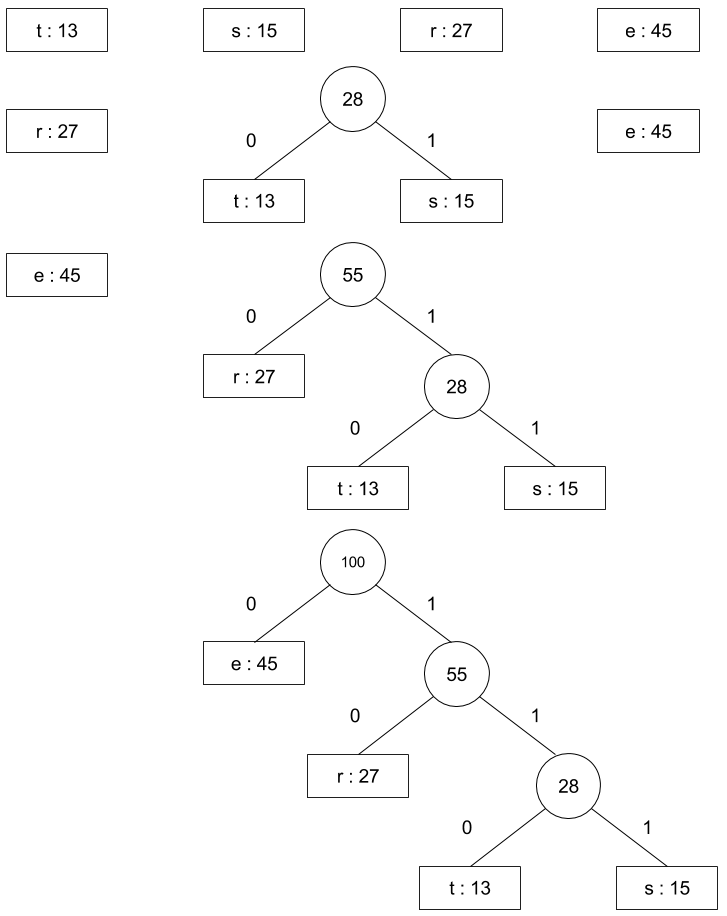
\includegraphics[scale=0.47]{images/huffman}
\centering %centering the image
\caption{Huffman-tre}
\label{fig:huffman}
\end{figure}
\end{boxed}
\newpage
\section{Trær}
\begin{figure}[H]
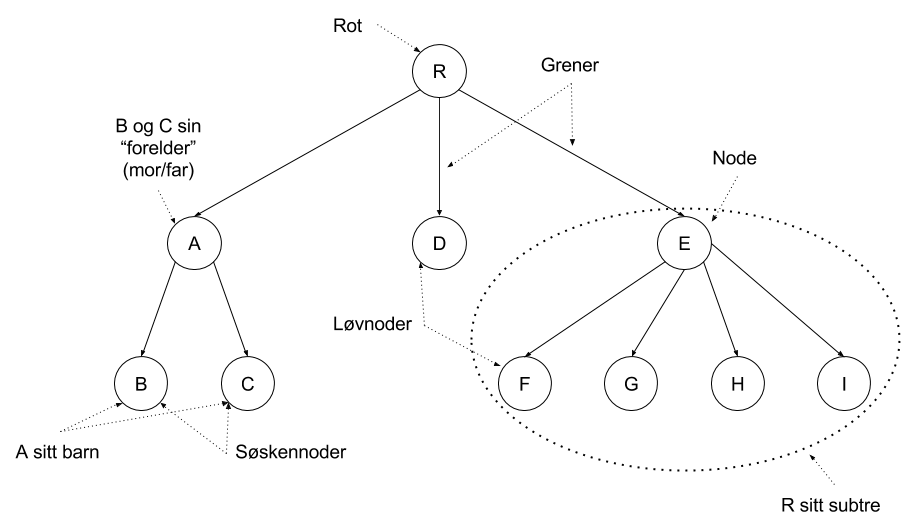
\includegraphics[scale=0.5]{images/traer}
\centering %centering the image
\caption{Tre}
\label{fig:trær}
\end{figure}

\begin{itemize}
    \item \textbf{Nivå for node} er antall grener som må passeres f.o.m. rot t.o.m. noden. Merk at rotnoden er på nivå 0.
    \item \textbf{Nodegrad} er antall barn (som er det samme som antall subtrær/undertrær) en node har.
    \item \textbf{Fritt tre} er at grenene ikke har retning, så alle nodene kan oppfattes som rotnode.
    \item \textbf{Rettet tre} vil si at grenene har retning, som i Figur \ref{fig:trær}.
    \item \textbf{Ordnet tre} vil si hvordan subtrærne/barna er ordnet i forhol til hverandre. Hvis det er viktig at A er til venstre, D i midten og E til høyre, er det et ordnet tre. Hvis rekkefølgen ikke har noe å si er det et uordnet tre.
    \item \textbf{Løvnode} er er node uten barn.
    \item \textbf{Indre node} er en node med barn.
    \item \textbf{Trehøyde} er maks antall grener som kan passeres f.o.m. rot t.o.m. løvnode.
    \item \textbf{$k$-grad-tre} vil si et tre der hver node kan ha maks $k$ barn. Posisjonen til barna er viktige.
    \item \textbf{Fullt $k$-grad-tre} er et $k$-grad-tre der alle indre noder har $k$ barn.
    \item \textbf{Komplett $k$-grad-tre} vil si et $k$-grad-tre der alle indre noder har $k$ barn, og enhver løvnode ligger på nivå $h$ eller $h - 1$, hvor $h$ er dybden (altså enten nederst i treet eller nest nederst). Antall noder på dybde $h$ er $k^h$. Trehøyden er $log_k n$ der $n$ er antall løvnoder.
\end{itemize}

\subsection{Implementasjon}
Hvordan vi implementerer en trestruktur avhenger av om vi har fast antall barn (f.eks. binære trær) eller variabelt antall barn (f.eks. B-trær).
\\\\
For hver av variantene har vi tatt med kjøretiden til to vanlige operasjoner:
\begin{itemize}
    \item finne forelder til en node
    \item finne barn nummer \textit{i} til en node
\end{itemize}

\noindent I generelle trær med fast antall barn har hver node er et objekt med en verdi, en peker til hver av barna og en peker til far.
\\\\
I generelle trær med variabelt antall barn er det to alternativer. Alternativ 1 er at hver node er et objekt med en verdi, en peker til sitt første barn (lengst til venstre), en peker til far og en til sin nærmeste bror til høyre for seg. I alternativ 2 utnytter vi at alle noder i et tre (untatt roten) har nøyatig én far. Vi lager en array. På plass nr \textit{i} står faren til node nummer \textit{i}, eller en peker til denne. Det blir da lett å finne faren, men for å finne barna til node \textit{i}, må vi søke gjennom arrayen etter tallet \textit{i}.

\begin{figure}[H]
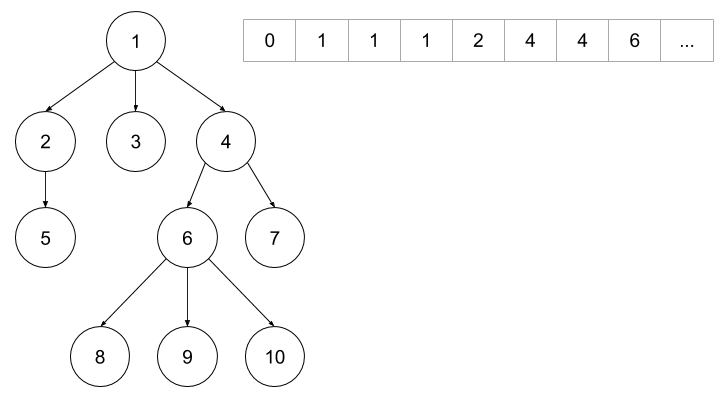
\includegraphics[scale=0.6]{images/fedrearray}
\centering %centering the image
\caption{Figuren viser et tre og den tilsvarende "fedrearrayen". Arrayen vil ha lke mange elementer som det er noder.}
\label{fig:fedrearray}
\end{figure}

\noindent Alternativ 3 er å lagre nodene i en array. HVert element i arrayen inneholder et objekt med verdien til noden og pekere til en lenket liste. Den lenkede listen inneholder pekere til barna.

\begin{figure}[H]
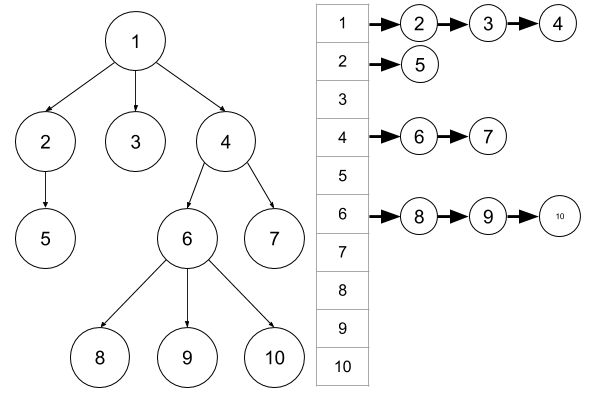
\includegraphics[scale=0.6]{images/alernativ3}
\centering %centering the image
\caption{Figuren viser alternativ 3.}
\label{fig:alternativ3}
\end{figure}

\subsection{Binære trær}
Binære trær er egentlig et 2-grad-tre, men dette navnet blir aldri brukt. Hver node har altså maks to barn og ordningen av høyre- og venstrebarn er viktig. Hver node er et objekt med en verdi, en peker til hver av barna og en peker til faren.

\begin{figure}[H]
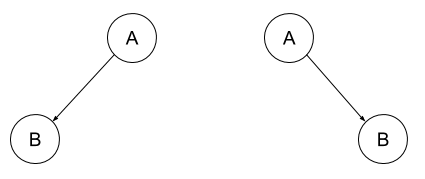
\includegraphics[scale=0.6]{images/binaeretraer}
\centering %centering the image
\caption{Disse to trærne er forskjellige!}
\label{fig:binaeretraer}
\end{figure}

\subsubsection{Binære søketrær}
Et binært søketre er bygget som et binært tre, men det er i tillegg organisert slik at verdien til venstre barn er mindre eller lik verdien til far mens verdien til høyre barn er større. Det betyr at for alle noder gjelder at alle verdiene til nodene i venstre subtre er lavere og alle i høyre er høyere enn verdien til noden selv. 

\begin{figure}[H]
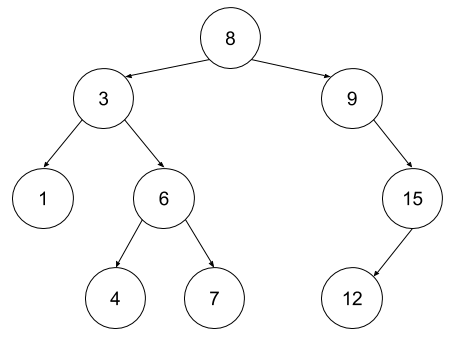
\includegraphics[scale=0.6]{images/binaeresoeketraer}
\centering %centering the image
\caption{Binært søketre}
\label{fig:binaeresoeketraer}
\end{figure}

\noindent Poenget er at med denne organiseringen er det vanligvis ganske kjapt å finne fram til ønsket node. Hvor lang tid det tar avhenger imidlertid av hvor heldig vi er med rekkefølgen nodene settes inn i. Hvor lang tid det tar å finne et element i verste tilfelle avhenger direkte av høyden til treet.
\\\\
\textbf{Innsetting av node}\\
Innsetting av noder i et binært tre er enkelt. Det er bare å passe på å overholde kriteriene for et binærtre. Vi starter alltid ved roten. Dersom treet ikke har noen rot, dvs. treet ikke er påbegynt, settes vår node til å være rotnoden. Ellers sjekker vi for hver nye node vi kommer til om verdien til noden vi skal sette inn er større eller mindre enn verdien til denne noden. Dersom den er mindre, går vi til venstre, ellers går vi til høyre. Vår node kan settes inn på første tomme plass vi kommer til.

\begin{figure}[H]
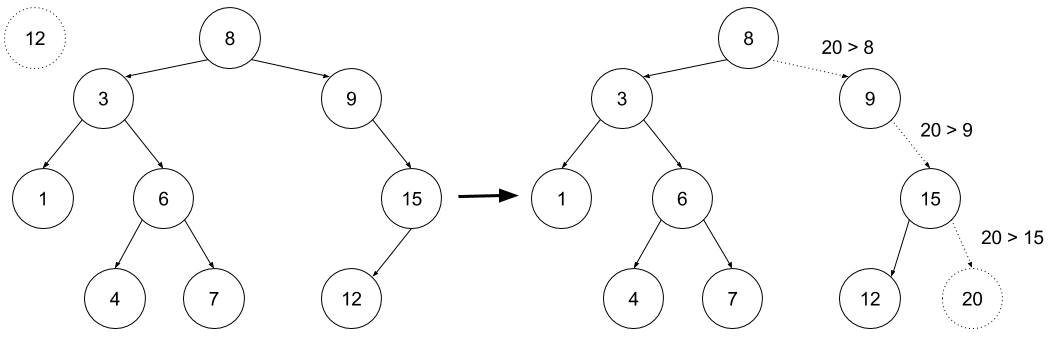
\includegraphics[scale=0.45]{images/innsettingnode}
\centering %centering the image
\caption{Sette inn node i binærtre}
\label{fig:innsettingnode}
\end{figure}

\noindent\textbf{Fjerning av node}\\
Vi har tre muligheter:
\begin{enumerate}
    \item \textbf{Noden vi skal fjerne har ingen barn.}\\ Vi kan da bare fjerne noden.
    \item \textbf{Noden vi skal fjerne har bare et barn.}\\ Vi kan da bare ta ut noden, og la barnet overta nodens far.
    \item \textbf{Noden vi skal fjerne har to barn.}\\ De to foregående tilfellene var enkle. Det er denne også, hvis man ser trikset. Spørsmålet vi må stille er: Hvilken annen node kan erstatte vår node, dvs. ta dens plass i treet? Det må være en med verdi større eller lik alle verdier i venstre subtre eller en med verdi mindre enn alle i høyre subtre. \newline \newline
    En løsning er å velge den noden med størst verdi i venstre subtre. Den finner du ved å gå til venstre barn og holde til høyre i hvert kryss videre nedover. Når du kommer til løvnoden har du funnet den du leter etter. \newline\newline
    En annen løsning er å velge den noden med minste verdi i høyre subtre. Helt tilsvarende går du da til høyre barn og holder til venstre i alle kryss helt til du når denne løvnoden.
    \newline\newline
    En av disse nodene kan klippes av og settes inn i stedet for den noden vi vil fjerne.
\end{enumerate}

\begin{figure}[H]
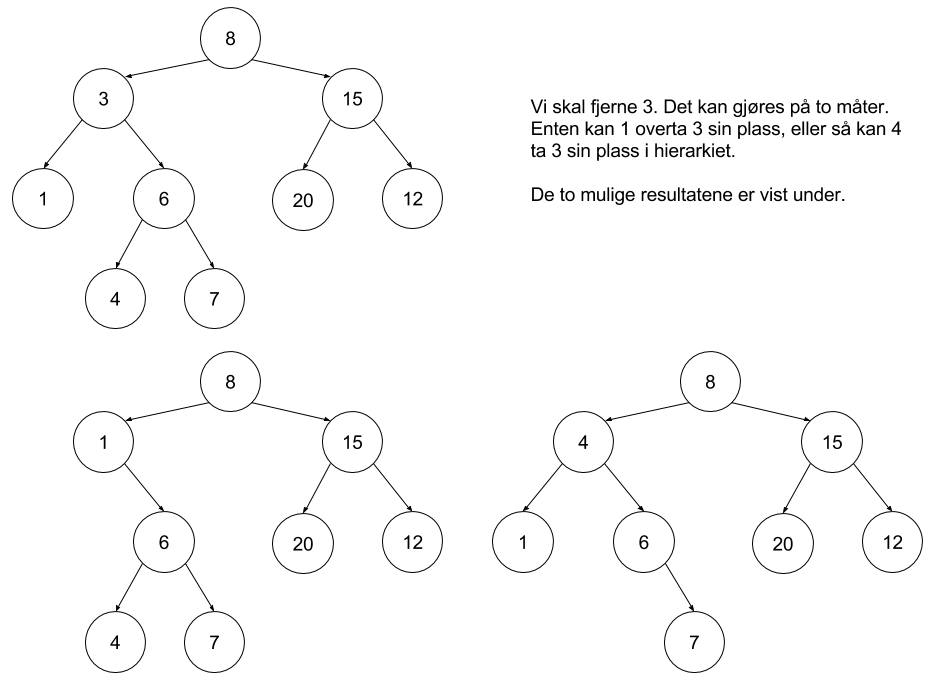
\includegraphics[scale=0.45]{images/fjernebarn}
\centering %centering the image
\caption{Fjerne barn}
\label{fig:fjernebarn}
\end{figure}

\subsection{Traversering}\\
Å traversere et tre eller en graf er et fint ord for å gå gjennom treet eller grafen. Her gir vi dere noen rekursive forklaringer på noen systematiske måter dette kan gjøres på.

\begin{itemize}
    \item \textbf{Prefiks:} Først utføres operasjonen på rotnoden, deretter prefikstraverseres venstre subtre (hvis det eksisterer) og til slutt prefikstraverseres høyre subtre (hvis det eksisterer). DFS. \textit{Kjører båt ved land, første man møter på.}
    \begin{figure}[H]
    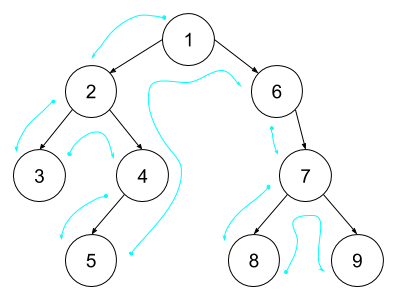
\includegraphics[scale=0.45]{images/prefiks}
    \centering %centering the image
    \caption{Prefikstraversering}
    \label{fig:prefiks}
    \end{figure}
    \item \textbf{Infiks:} Først infikstraverseres venstre subtre, deretter utføres operasjonen på rotnoden og til slutt infikstraverseres høyre subtre. DFS. 
    \begin{figure}[H]
    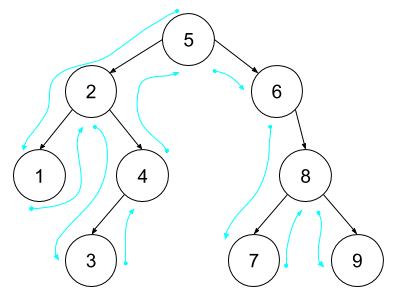
\includegraphics[scale=0.45]{images/infiks}
    \centering %centering the image
    \caption{Infikstraversering}
    \label{fig:infiks}
    \end{figure}
    \item \textbf{Postfiks:} Først postfikstraverseres venstre subtre, deretter høyre og til slutt utføres operasjonen på rotnoden. DFS. \textit{Siste på hver gren merkes.}
    \begin{figure}[H]
    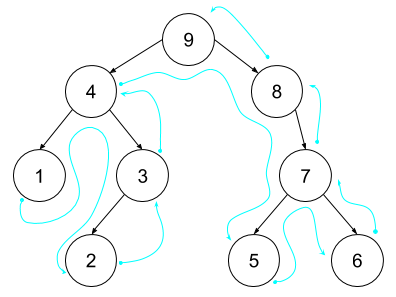
\includegraphics[scale=0.45]{images/postfiks}
    \centering %centering the image
    \caption{Postfikstraversering}
    \label{fig:postfiks}
    \end{figure}
    \item \textbf{Nivå:} Vi utfører først operasjonen på roten. Deretter tar vi for oss én og én rad på vei nediver, vanligvis fra venstre mot høyre. BFS. \textit{Merker fra venstre til høyre på hver rad.}
    \begin{figure}[H]
    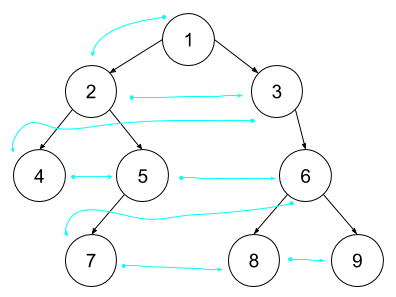
\includegraphics[scale=0.45]{images/nivaa}
    \centering %centering the image
    \caption{Nivåtraversering}
    \label{fig:nivå}
    \end{figure}
\end{itemize}

\begin{boxed}
\begin{itemize}
    \item \textbf{Preorder}: Her printer man ut nodens verdi før dens barn, venstre og deretter høyre. 
    \begin{itemize}
        \item Eksempel fra figuren under: 10, 6, 3, 2, 1, 4, 5, 8, 7, 9, 13, 11, 12, 18, 15, 14, 16, 17
    \end{itemize}
    \item \textbf{Inorder}: Her printer man venstre barn, noden, og deretter høyre barn (om ikke det er noe venstre barn, print noden før høyre barn)
    \begin{itemize}
        \item Eksempel fra figuren under: 1, 2, 3, 4, 5, 6, 7, 8, 9, 10, 11, 12, 13, 14, 15, 16, 17, 18
    \end{itemize}
    \item \textbf{Postorder}: Her printer man nodens verdi etter man har printet venstre og høyre barn
    \begin{itemize}
        \item Eksempel fra figuren under: 1, 2, 5, 4, 3, 7, 9, 8, 6, 12, 11, 14, 17, 16, 15, 18, 13, 10
    \end{itemize}
\end{itemize}

\begin{figure}[H]
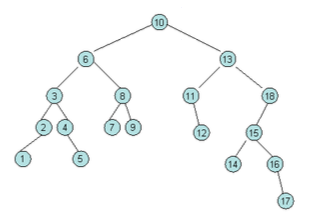
\includegraphics[scale=0.8]{images/tregraf}
\centering %centering the image
\caption{Tre}
\label{fig:tregraf}
\end{figure}
\end{boxed}

\subsection{Minimale spenntrær}
Som vi vet er et tre en forbundet graf uten sykler. Et \textbf{spenntre} er en subgraf av en graf \textit{G} som inneholder \textit{V - 1} kanter. Et \textbf{minimalt spenntre}, forkortet MST, av en vektet graf \textit{G} er et spenntre av \textit{G} som er slik at summen av kostnadene til kantene som inngår i treet, er minimal (det vil si at det ikke er mulig å lage andre spenntrær men mindre kantkostnader). Et MST er ikke nødvendigvis unikt – den kan altså finnes flere MST'er for samme graf.

\subsubsection{Prim}
Prinsippet med Prims algoritme er å alltid begynne med en tilfeldig node. I hvert steg ser man på alle kanter som forbinder en node som er med i treet man har bygget hittil med en node som ikke er med, og velger den kanten med minst kostnad. Dette gjøres ved å ha de ubrukte nodene i en prioritetskø, og markere hver node med den korteste kanten som forbinder den med en node i treet. Når alle nodene er med i treet, har du funnet et minimalt spenntre.
\\\\
Altså den mengden med kanter som minimerer summen av vekter samtidig som grafen er sammenhengende. Det minimale spenntreet reflekterer ikke nødvendigvis de faktisk korteste veiene fra en node til en annen.

\subsubsection{Kruskal}
Prinsippet med Kruskals algorimte er å sortere alle kantene etter kostnad, og se på kantene i stigende rekkefølge. Ta en kant (og nodene den går mellom) i spenntreet med mindre kanten ville ha laget en sykel. Fortsett til det ikke er flere kanter som kan legges til. Ideen er enkel, men for at algoritmen skal bli effektiv trenger man en avansert datastruktur som kalles \textit{disjoint set} for raskt å kunne finne ut om en kant vil danne en sykel eller ikke. Derfor anbefales Prim når man skal implementere en MST-algoritme selv.
\newpage
\section{Problemkompleksitet}
Det finnes mange klasser av problemer. P, NP, NPC og NP-Hard er fire slike klasser.

\subsection{NP (Non-deterministic Polynomial}
Mengden av de problemene der gyldigheten av en gjettet løsning kan testes i polynomisk tid.

\subsection{P (Polynomial}
Mengden av de problemene vi vet kan løses i polynomisk tid. Det vil si de som har ''worst case'' kjøretid på $O(n^k)$, hvor \textit{k} er en konstant og \textit{n} er størrelsen på input. Det er opplagt at disse er med i mengden NP. Det er slike problemer dette kurset går ut på å løse. 

\subsection{NPC (NP-komplett)}
Enkelt forklart er dette samlingen av de vanskeligste problemene i NP. Hvis det finner en polynomisk løsning for et problem i NPC, finnes det polynomiske løsninger for alle problemer i NP. Dette er definisjonen på et NP-komplett problem. Alle NP-komplette problemer kan nemlig omformes til hverandre, så dersom vi finner en polynomisk løsning på ett av disse problemene, har vi løst dem alle (og $NP = P$, siden NPC var de vanskeligste problemene i NP, og det viste seg at de også kunne løses i polynomisk tid). Det motsatte gjelder også; hvis et av problemene i NPC viser seg å være uløsbart i polynomisk tid, er alle det. Hittil har man kun funnet eksponentielle løsninger av NPC-problemer.
\\\\
I likhet med andre ''komplette'' problemer i andre problem-klasser er altså NPC-problemene de vanskeligste som finnes i klassen. I prinsippet er de også ett og samme problem, da alle kan reduseres til det samme problemet i polynomisk tid. (Det ville også vært meningsløst å si at flere lignende problemer er "det vanskeligste"). Her kan det være verdt å få med seg at hvis et problem A kan reduseres (omformes) til et problem B på mindre tid enn (eller like mye tid som) det tar å løse B, kan B sies å være minst like vanskelig som A (har vi en algoritme for å løse B, kan vi bruke den til å løse A, men det er ikke sikkert at en algoritme for A kan løse B).
\\\\
Foreløpig er det ikke funnet noen algoritme som kan løse NPC-problemer i polynomisk tid, men det er jeller ikke bevist at en slik løsning ikke finnes. Dette er antakeligvis det største uløste problemet innen informatikkens verden, og den som enten klarer å finne en polynomisk løsning eller klarer å bevise at dette ikke er mulig vil bli en av verdens mest kjente vitenskapsmenn (eller kvinner).
\\\\
\textbf{NP-hard} er mengden av de problemene som alle problemer i NP kan reduseres til i polynomisk tid. Disse problemene trenger ikke nødvendigvis ligge i NP. NP-hard er ikke pensum, men begrepet vil sikkert dukke opp.

\subsection{SAT-problemet}
Men hvordan vie at et problem er NPC? Det høres i utgangspunktet umulig ut, med heldigvis finnes det teoremer som sier at SAT-problemet er i NPC. Sat går ut på at vi har en boolsk krets eller boolsk nettverk med AND-, OR- og NOT-porter, og så ønsker vi å finne ut om der eksisterer et sett med inputverdier (0er/false og 1ere/true) som gjør at outputen blir 1 (true). Det vi må vise er at alle problemer i NP kan reduseres til SAT-problemet i polynomisk tid.

\subsubsection{Andre kjente NPC-problemer}
SAT-problemet er ikke veldig enkelt å jobbe med. Det er ofte enklere å sammenligne problemet med andre kjente NPC-problem. Vi skal presentere noen for dere her. Hvis dere blir spurt om å vise at et problem er NPC, kan dere bruke en av disse å sammenligne med.
\\\\
\textbf{Lengste vei:} Vi har sett på algoritmer som finner korteste vei i grafer uten negative sykler med polynomisk kjøretid. Men for generelle grafer blir det verre. Å finne korteste eller lengste vei i en graf er NPC hvis man ikke har noen begrensninger på kantvektene (slik som for eksempel ingen negative kanter for å unngå sykler). Men, akkurat som at korteste-vei-problemet der man ikke har negative sykler som en del av P, gjelder det samme for lengste-vei-problemet for grafer uten positive sykler. Dette er fordi man kan gange alle kantvekter med $-1$ og dermed få et ekvivalent korteste-vei-problem.
\\\\
\textbf{Klikk:} En klikk er en komplett subgraf av grafen $G$. Det vil si dersom en delmengde av nodene i $G$ har forbindelse til alle andre i denne delmengden, har vi en klikk (alle kjenner alle i en klikk). Størrelsen på klikken er antall noder som er med. Spørsmålet "Eksisterer det en klikk av en gitt størrelse $k$" gir oss et NPC-problem.
\\\\
\textbf{Hamiltonsykel:} Vi kan finne en Euler-sti (kantene benyttes en og bare en gang når vi traverserer grafen, uten å hoppe) i polynomsik tid, men å bestemme om en graf har en Hamilton-sykel er et NPC-problem. (I en Hamilton-sykel besøkes nodene en og bare en gang langs en sammenhengende vei gjennom grafen, dvs. vi har en enkel sykel gjennom alle nodene i grafen.)
\\\\
\textbf{Travelling Salesman Problem (TSP):} Vi har en handelsmann som skal besøke $n$ byer. Han skal bare innom hver by en gang og ønsker å gjøre rundturen så billig som mulig. Poenget her er altså å finne en minimal Hamiltonsykel. Eller for å være helt korrekt er problemet å finne ut om det eksisterer en rute som er $\leq$ en gitt verdi.

\subsection{Hvordan bevise at et problem er P, NP, og NPC?}
For å bevise at et problem er med i P (dv. kan løses i polynomisk tid), må du finne en algoritme som løser problemet i polynomisk tid. 
\\\\
For å bevise at et problem er med i NP, må du finne en algoritme som tester om en gjettet løsning er korrekt. Denne må kjøre i polynomisk tid.
\\\\
For å bevise at et problem er med i NPC, må du vise at det er med i NP, og at det er minst like vanskelig som et annet problem du vet er i NPC. Det finnes bøker med lister over kjente NPC-problemer. Måten du gjør det på er å transformere det kjente problemet til ditt problem eller en enklere utgave av ditt problem. Transformasjonen må kunne gjøres i polynomisk tid. Det er på tide med et eksempel.

\begin{boxed}
Vi må først vise at TSP er med i NP. Problemet er å finne ut om det eksisterer en rute som er $\leq$ $x$ kilometer. På mystisk vis gjettes vi på det beste veivalget. Det er innlysende at vi med letthet (dvs. i polynomisk tid) kan finne ut om denne veien er kortere eller like lang som $x$. (Vi trenger bare ¨å slå opp avstandene og addere de sammen.) Dette vider at TSP er med i NP.
\newline
\newline
Nå kan vi vise at TSP er med i NCP. Vi tar utgangspunkt i Hamiltonsykelproblemet. La oss si at nodene i grafen er byer og kantene er veier. Vi setter kostnaden på kantene til å være 1. Eksisterer det en tur som har lengde $\leq$ antall noder? Dette er et ``travelling salesman problem`` av enkleste sort. Poenget er at spørsmålet kunne like gjerne vært: Finnes det en Hamiltonsykel i grafen? Dette er et problem vi gikk ut i fra er NPC.
\newline
\newline
Av sammenligningen skjønner vi at dersom vi finner en algoritme for å løse vårt problem (TSP), vil denne også kunne løse Hamiltonsykel-problemet. Altså kan vi konkludere med at TSP er NPC.
\end{boxed}
\newpage
\section{Kjøretider til pensumalgoritmer}
\begin{table}[]
\centering
\label{oversikt}
\begin{tabular}{|c|l|l|l|l|}
\hline
\multirow{\textbf{Problem}} & \multirow{\textbf{Algoritme}} & \multicolumn{3}{c|}{\textbf{Kjøretid}}    \\ \cline{3-5} & & \multicolumn{1}{c|}{\textbf{BC}} & \multicolumn{1}{c|}{\textbf{AC}} & \multicolumn{1}{c|}{\textbf{WC}} \\ 
\hline
\multirow{\textbf{Sortering}} & Insertion sort  & $\theta(n)$  & $\theta(n^2)$ & $\theta(n^2)$ \\ \cline{2-5}
 & Bubble sort & $\theta(n)$ & $\theta(n^2)$ & $\theta(n^2)$ \\ \cline{2-5} 
 & Merge sort & $\theta(n lg (n))$ &  $\theta(n lg (n))$ & $O(n lg (n))$\\ \cline{2-5} 
 & Heap sort & $O(n lg (n))$ & $O(n lg (n))$ &$O(n lg (n))$\\ \cline{2-5} 
 & Quicksort & $\theta(n lg (n))$ & $O(n lg (n))$ & $\theta(n^2)$ \\ \cline{2-5} 
 & Counting sort & - & $\theta(n)$ & $\theta(k + n)$ hvis $k = O(n)$ \\ \cline{2-5} 
 & Radix sort & - & $\theta(d(k + n))$ & - \\ \cline{2-5} 
 & Bucket sort & -  & $\theta(n)$ & -\\ \hline
\multirow{\textbf{Grafer/trær}} & Topologisk sortering & - & $\theta(|V|+|E|)$ & -\\ \cline{2-5} 
 & DFS  & - & $\theta(|V|+|E|)$ & -\\ \cline{2-5} 
 & BFS & - & $O(|V|+|E|)$ & - \\ \cline{2-5} 
 & Prim & $O(E lg(V))$ & $O(E lg(V))$ & - \\ \cline{2-5} 
 & Kruskal & $O(E lg(V))$ & $O(E lg(V))$ & -\\ \cline{2-5} 
 & Binærsøk & $O(lg n)$ & - & $O(lg n)$\\ \hline
\multicolumn{1}{|l|}{\multirow{\textbf{Korteste vei}}} & Bellman-Ford & - & $O(|V|*|E|)$ & -\\ \cline{2-5} 
\multicolumn{1}{|l|}{} & Dijkstra & $O(|E| lg (|V|))$ (bin-heap) & $O(|V|^2)$ (array) & -\\ \cline{2-5} 
\multicolumn{1}{|l|}{} & DAG-Shortest-Path & - & $\theta(|V|*|E|)$ & \\ \cline{2-5} 
\multicolumn{1}{|l|}{} & Floyd-Warshall & - & $\theta(|V|^3)$ & -\\ \hline
\multicolumn{1}{|l|}{\multirow{\textbf{Flyt}}} & Ford-Fulkerson & - & $O(E|f^*|)$  &  $f^*$ = maks flyt i G\\ \cline{2-5} 
\multicolumn{1}{|l|}{} & Edmonds-Karp & - & $O(VE^2)$ & -\\ \hline
\multicolumn{1}{|l|}{\textbf{Grådig}} & Huffmann & $O(n lg (n))$ &- &-\\ \hline
\end{tabular}
\end{table}

\subsection{Sortering og velging}
\subsubsection{INSERTION SORT}
Nummerense vi sil sortere kalles \textit{nøkler}. Er effektiv for å sortere små mengder tall. Fungerer slik amge sorterer en korthånd. Bruker sammenligning. Sorterer \textit{in-place}.
\subsubsection{MERGE SORT}
\subsubsection{QUICKSORT}
\subsubsection{RANDOMIZED-QUICKSORT}
\subsubsection{COUNTING SORT}
\subsubsection{RADIX SORT}
\subsubsection{BUCKET SORT}
\subsubsection{HEAPSORT}
\subsection{Heap-operasjoner}
\subsection{Graf-operasjoner}
\subsubsection{TOPOLOGISK SORTERING}
\subsubsection{BFS}
\subsubsection{DFS}
\subsection{Korteste vei}
\subsubsection{BELLMAN-FORD}
\subsubsection{DAG-SHORTEST-PATH}
\subsubsection{DIJKSTRA}
\subsubsection{FLOYD-WARSHALL}
\subsection{Flytalgoritmer}
\subsubsection{FORD-FULKERSON}
\subsubsection{EDMONDS-KARP}
\subsection{Grådige algoritmer}
\subsubsection{HUFFMAN}
\subsection{Andre algoritmer}
\newpage
\section{Lineær programmering}
Lineær programmering er spesielt nyttig i det som kalles \textbf{optimeringsteori}. Dette går ut på å enten minimere eller maksimere en lineær funksjon med en hel del krav.

\begin{boxed}
Anta at Gløshaugen har komponert et nytt fag som kalles ``\textbf{part.kont}```som består av 50\% partikkelfysikk og 50\% kontorlandskap. Dette faget er obligatorisk for deg, og du skal levere to semesteroppgaver, en for hver del. Det gis karakter for begge. Men fordi du synes dette faget er tullete og du har mye annet å gjøre, ønsker du å bruke så lite tid på faget som mulig samtidig som du skal bestå. La oss kalle tiden du bruker på partikkelfysikk for $x_1$, og tiden på kontorlandskap $x_2$. Du vet at det vil være to sensorer, en tørr professor og en økonom. Du regner med at du får 5 poeng per arbeidstime fra den tørre professoren og 2 fra økonomen for oppgaven i partikkelfysikk, mens for kontorlandskap får du 1 poeng per arbeidstime fra den tørre professoren og økonomen gir 4. Vi oppsummerer dette i en tabell.

\begin{table}[H]
    \caption{Poeng per arbeidstime}
    \label{tab:kjoretideks}
    \centering
    \begin{tabular}{|L{10em} | L{10em}|L{10em}|}
        \hline
        \rowcolor[HTML]{303F9F}
        \textbf{\textcolor{white}{}} & \textbf{\textcolor{white}{Tørr professor}} & \textbf{\textcolor{white}{Økonom}}\\
        \rowcolor[HTML]{E6E6E6}
        Partikkelfysikk & 5 & 2\\
        Kontorlandskap & 1 & 4\\
         \hline
    \end{tabular}
\end{table}

Poenget er nå at for å stå må du få minst 40 poeng for hver oppgave. For å sikredeg litt, krever du at du skal ha stått hos begge sensorene. Da kan vi sette opp et ligningssystem som ser slik ut:
\newline
\newline
Minimér:
\begin{center}
$x_1 + x_2$
\end{center}
Hvor:
\begin{center}
$5x_1 + x_2 \geq 40$ \newline
$2x_1 + 4x_2 \geq 40$ \newline
$x_1, x_2 \geq 0$
\end{center}
Den siste ligningen viser bare at tiden vi bruker ikke kan være negativ. Uttryket $x_1 + x_2$ er en lineær funksjon som vi vil skal få en størst mulig verdi uten at verdiene av variablene bryter noen av ulikhetene. Dette kalles for et linæert program, og det kan løses med lineær programmering.
\end{boxed}

\noindent Når man skal løse et problem som dette finnes det flere avanserte metoder. Den eneste som nevnes i boken er \textbf{simplex-metoden}, som minner litt om Gauss-eliminasjon. Den tar først og oversetter alle problemene til sin egen standardform, slik at det generelt kan skrives om:
\newline
\newline
Maksimér:
\begin{center}
$\sum\limits_{j=1}^n c_j x_j$
\end{center}
Hvor:
\begin{center}
$\sum\limits_{j=1}^n a_{ij} x_j \leq b_i$ for $i = 1, 2, ...m$ \newline
$x_j \geq 0$ for $j = 1, 2, ..., n$
\end{center}

Som man kanskje aner, så er det ekstremt nyttig å løse slike former for problemer. Vi skal ikke her vise hvordan simplex-metoden fungerer (det er heller ikke pensum), men interesserte anbefales å se på dette, i kapittel 29.3 i læreboken. Det som derimot \textit{er} pensum er å kunne formulere problemer slik at de kan løses med lineær programmering - det vil si å sette opp et lineært program og begrunne hverfor løsningen av det lineære programmet vil være en løsning av problemet.
\\\\
Et \textit{lineært program} består av følgende:
\begin{enumerate}
    \item Et lineært uttrykk som skal maksimeres eller minimeres, kalt den \textit{objektive funksjonen}
    \item En samling lineære ulikheter og/eller ligninger, som fungerer som restriksjoner på variablene i den objektive funksjonen.
\end{enumerate}

\noindent Med en gang man kan skrive om et problem til et lineært program, finnes det en rekke glupe algoritmer for å løse dette på. Simplex-metoden er én måte å gjøre det på, med den er gammel, og idag brukes langt mer raffinerte metoder. Vi skal her vise lett to problemer vi har vært borte i som kan oversettes til lineær programmering.

%sett inn eksempler her
\newpage
\section{Formler}
\subsubsection{Håndtrykksformelen}
Dette er én av to enkle men viktige formler som stadig dukker opp når man skal
analysere algoritmer. Formelen er:
\begin{center}
$\sum\limits_{i=0}^{n-1} i = \frac{n(n-1)}{2}$
\end{center}

\noindent Den kalles gjerne håndtrykksformelen, fordi den beskriver antall håndtrykk som
utføres om $n$ personer skal hilse på hverandre. Vi kan vise dette ved å telle antall
håndtrykk på to ulike måter. De to resultatene må da være like.
\\\\
\textbf{Telling 1:} La oss se på personene én etter én. Første person hilser på alle de
andre $n − 1$ personene. Andre person har allerede hilst på første person, men
bidrar med $n − 2$ nye håndtrykk ved å hilse på de gjenværende. Generelt vil
person $i$ bidra med $n − i$ nye håndtrykk, så totalen blir
\begin{center}
$(n − 1)$ + $(n − 2)$ + · · · + $2 + 1 + 0 $
\end{center}

\noindent Om vi snur summen, så vi får $0 + 1$ + · · · + $(n − 1)$, så er dette den venstre siden
av ligningen. Dette oppstår typisk i algoritmer der vi utfører en løkke gjentatte
ganger, og antall iterasjoner i løkka øker eller synker med 1 for hver gang, slik:

\begin{lstlisting}
for i = 1 . . n − 1
    for j = i + 1 . . n
        i tar j i h˚anden
\end{lstlisting}

\noindent Telling 2: Vi kan også telle på en mer rett frem måte: Hver person tar alle de
andre i hånden, og inngår dermed i $n − 1$ håndtrykk. Hvis vi bare teller hver
enkelt person sin halvdel av håndtrykket, får vi altså $n(n − 1)$ halve håndtrykk.
To slike halve håndtrykk utgjør jo ett helt, så det totale antallet håndtrykk blir
den høyre siden av ligningen, nemlig $n(n − 1)/2$.
Man kan også gjøre om en sum av denne typen ved å brette den på midten, og
legge sammen første og siste element, nest første og nest siste, etc. Vi får da
\begin{center}
$(n − 1 + 0) + (n − 2 + 1) + (n − 3 + 2) + . . .$
\end{center}

\noindent Hvert ledd summerer til $n−1$, og det er $n/2$ ledd. Mer generelt er summen av en
aritmetisk rekke (der vi øker med en konstant fra ledd til ledd) lik gjennomsnittet
av første og siste ledd, multiplisert med antallet ledd i rekken.

\subsection{Utslagsturneringer}
Dette er den andre av de to sentrale formlene:
\begin{center}
$\sum\limits_{i=0}^{h-1} 2^i = 2^h - 1$
\end{center}
Det vil si, de første toerpotensene summerer til én mindre enn den neste. En
måte å se dette på er av totallssystemet, der et tall $a = 11$ · · · $1$ med $h$ ettall
etterfølges av tallet $b = 100 · · · 0$, som består av ett ettall, og $h$ nuller. Her er
\begin{center}
$a = 20 + 21 + · · · + 2h−1 og b = 2h$, så a = b − 1.
\end{center}

\noindent Et grundigere bevis kan vi få ved å bruke samme teknikk som før, og telle
samme ting på to ulike måter. Det vi vil telle er antall matcher i en utslagsturnering
(knockout-turnering), det vil si, en turnering der taperen i en match er
ute av spillet. Dette blir altså annerledes enn såkalte round robin-turneringer,
der alle møter alle – for dem kan vi bruke håndtrykksformelen for å finne antall
matcher, siden hver match tilsvarer ett håndtrykk.

%se metode 1 og 2 i heftet

\subsection{Reduksjoner}
%se heftet

\end{document}